\documentclass[10pt,journal,compsoc,twocolumn,twoside]{IEEEtran}
% \def\BibTeX{{\rm B\kern-.05em{\sc i\kern-.025em b}\kern-.08em
%     T\kern-.1667em\lower.7ex\hbox{E}\kern-.125emX}}

\usepackage{amsmath}
\usepackage{bm}
\usepackage{nicefrac}
\usepackage{booktabs}
\usepackage{array}
\usepackage{multirow}
\usepackage{threeparttable}
\usepackage{makecell}
\usepackage[procnumbered,ruled,vlined,linesnumbered]{algorithm2e}
\usepackage{siunitx}
\usepackage{stfloats}
\usepackage{graphicx}
\usepackage{subfigure}
\usepackage{hyperref}
\usepackage{array}
\usepackage{epstopdf}
\usepackage{balance}
\usepackage{tabularx}
\usepackage{stfloats}
\usepackage{lipsum}

\newtheorem{problem}{Problem}
\newtheorem{theorem}{Theorem}[section]
\newtheorem{corollary}[theorem]{Corollary}
\newtheorem{lemma}[theorem]{Lemma}
\newtheorem{definition}[theorem]{Definition}
\newtheorem{fact}[theorem]{Fact}

% \newcommand{\proof}{{\bf Proof.}\hskip 0.3truecm}
% \newcommand{\endproof}{\quad \(\Box\)}

\newcommand{\defeq}{\stackrel{\mathrm{def}}{=}}
\newcommand{\setof}[1]{\left\{#1 \right\}}
% \newcommand{\sizeof}[1]{\left|#1 \right|}
\newcommand{\abs}[1]{\left|#1 \right|}
\newcommand{\mean}[1]{\mathbb{E}[#1]}
\newcommand{\ceil}[1]{\left\lceil#1\right\rceil}
\newcommand{\Abs}[1]{\left\Vert#1\right\Vert}
\newcommand{\trace}[1]{\mathrm{Tr}\left(#1\right)}

\newcommand{\bsym}[1]{\boldsymbol{#1}}
\newcommand{\myord}[1]{{#1}^{\rm{th}}}
\newcommand{\rea}{\mathbb{R}}
\newcommand{\gr}{\mathcal{G}}
\newcommand{\vecd}{\bsym{d}}
\newcommand{\veca}{\bsym{a}}
\newcommand{\vecb}{\bsym{b}}
\newcommand{\vece}{\bsym{e}}
\newcommand{\allone}{\bsym{1}}
\newcommand{\vecl}{\bsym{l}}
\newcommand{\vecv}{\bsym{v}}
\newcommand{\vecpi}{\bsym{\pi}}
\newcommand{\vecx}{\bsym{x}}

\newcommand{\pscr}{\mathscr{P}}

\newcommand{\lap}{\bsym{L}}
\newcommand{\matd}{\bsym{D}}
\newcommand{\mata}{\bsym{A}}
\newcommand{\matb}{\bsym{B}}
\newcommand{\matw}{\bsym{W}}
\newcommand{\matp}{\bsym{P}}
\newcommand{\matpcal}{\bsym{\mathcal{P}}}
\newcommand{\matf}{\bsym{F}}
\newcommand{\matfstar}{\bsym{F}^*}
\newcommand{\mati}{\bsym{I}}
\newcommand{\matq}{\bsym{Q}}
\newcommand{\matr}{\bsym{R}}
\newcommand{\mats}{\bsym{S}}
\newcommand{\matx}{\bsym{X}}
\newcommand{\maty}{\bsym{Y}}
\newcommand{\matz}{\bsym{Z}}
\newcommand{\matpi}{\bsym{\Pi}}

\newcommand{\lemref}[1]{Lemma~\ref{#1}}
\newcommand{\thmref}[1]{Theorem~\ref{#1}}
\newcommand{\probref}[1]{Problem~\ref{#1}}
\newcommand{\algoref}[1]{Algorithm~\ref{#1}}
\newcommand{\defref}[1]{Definition~\ref{#1}}
\newcommand{\secref}[1]{Section~\ref{#1}}
\newcommand{\tabref}[1]{Table~\ref{#1}}
\newcommand{\figref}[1]{Figure~\ref{#1}}

\newcommand{\edge}[2]{\langle #1, #2 \rangle}


\DeclareMathOperator*{\argmin}{arg\,min}
\DeclareMathOperator*{\argmax}{arg\,max}

\DontPrintSemicolon
\SetKw{KwAnd}{and}
\SetFuncSty{textsc}
\SetKwInOut{Input}{Input\ \ \ \ }

\SetKwInOut{Output}{Output}
\newcommand{\biophoto}[1]{\includegraphics[width=1in,height=1.25in,clip,keepaspectratio]{#1}}
\newcommand{\todo}[1]{{\bf \color{red} TODO: #1}}
\hyphenation{Exact-AGCM}

\begin{document}

\title{Absorbing Time of Random Walks\\ as a Node Group Centrality}
\author{Haisong~Xia,
    Wanyue~Xu~\IEEEmembership{Student Member,~IEEE},
    Zuobai~Zhang,
    Zhuoqing~Song,
    Zhongzhi~Zhang~\IEEEmembership{Member,~IEEE}
    \thanks{Haisong Xia, Wanyue Xu and Zhongzhi Zhang are with the Shanghai Key Laboratory of Intelligent Information Processing, School of Computer Science, Fudan University, Shanghai 200433, China; Zhongzhi Zhang is also with the Shanghai Engineering Research Institute of Blockchain, Shanghai 200433, China.}
}

\markboth{IEEE Transactions on Information Theory}
{Xia \MakeLowercase{\textit{et al.}}: Absorbing Time of Random Walks as a Node Group Centrality}

\IEEEtitleabstractindextext{
    \begin{abstract}
        For random walks on an undirected graph, the mean hitting time \(H_j\) from a vertex \(i\) chosen from the stationary distribution to the target vertex \(j\) can be used as a measure of importance for vertex \(j\), while the Kemeny constant \(K\) is the mean hitting time from a vertex \(i\) to a vertex \(j\) selected randomly according to the stationary distribution.
        Both quantities have found a large variety of applications in different areas.
        However, their high computational complexity limits their applications, especially for large networks with millions of vertices.
        In this paper, we first establish a connection between the two quantities, representing \(K\) in terms of \(H_j\) for all vertices.
        Subsequently, we extend the notion of mean hitting time to the case of multiple vertices, proposing a vertex group centrality called Absorbing Group Centrality (AGC).
        We then express these quantities in terms of either the pseudoinverse for graph Laplacian or the inverse for a SDDM matrix, based on which we develop an efficient algorithm that provides an approximation of \(H_j\) for all vertices and \(K\) in nearly linear time with respect to the edge number, with high probability.
        Moreover, we study the problem of finding a subset \(S\) of \(k\) vertices to minimize its AGC \(\manc{S}\), proving its NP-hardness.
        Based on the aforementioned algorithm, we provide another nearly linear greedy algorithm to solve the AGC minimization problem with a \(1-\frac{k}{k-1}\cdot\frac{1}{e}-\epsilon\) approximation factor for any error parameter \(\epsilon\in(0,1)\).
        Extensive experiment results on real-life and model networks validate both the efficiency and accuracy of our proposed algorithms.
    \end{abstract}

    \begin{IEEEkeywords}
        Random walk, hitting time, Kemeny constant, spectral algorithm, complex network, vertex centrality.
    \end{IEEEkeywords}
}

\maketitle

\IEEEdisplaynontitleabstractindextext

\IEEEpeerreviewmaketitle

\section{Introduction}\label{sec:intro}

\IEEEPARstart{A}{s} a powerful tool and method, random walks have found broad applications in various aspects.
Frequently cited examples include image segmentation~\cite{Le06}, random algorithm design~\cite{SaDi12}, collaborative recommendation~\cite{FoPiReSa07}, community detection~\cite{LaDeBa14}, among others.
A fundamental quantity related to random walks is hitting time~\cite{Lo93}, also called first-passage time~\cite{CoBeTeVoKl07}.
For a random walk on a graph, the hitting time \(H_{ij}\) from a vertex \(i\) to another vertex \(j\) is the expected time for the walker starting from \(i\) to visit \(j\) for the first time.
Hitting time is related to many problems and has been successfully applied to diverse areas, such as Hanoi problem with random move~\cite{WuZhCh11}, query suggestion~\cite{MeZhCh08}, and clustering algorithm~\cite{ChLiTa08}.

Except for the intrinsic interest of hitting time itself and its direct applications, many other relevant quantities related to random walks are encoded in or expressed in terms of this crucial quantity, for example, absorbing random-walk centrality~\cite{MaMagi15} (or Markov centrality~\cite{WhSm03}), Kemeny constant~\cite{Hu14} and random detour time~\cite{RaZh13}.
As the name implies, the absorbing random-walk centrality is a measure for the importance of vertices on a graph.
For a vertex \(j\), its absorbing random-walk centrality \(H_j\) is defined by \(H_j=\sum_{i} \rho(i) H_{ij}\), where \(\rho(\cdot)\) is the starting probability distribution over all vertices.
Different from the shortest-path based centrality measures, random-walk based centrality metrics include the contributions from essentially all paths~\cite{Ne05}, and thus have a better discriminating power.

For random walks on a graph with \(n\) vertices, the Kemeny constant \(K\) is defined as the expected time for the walker starting from one vertex to second vertex selected randomly from the graph according to the stationary distribution \(\vecpi=\left(\pi_1, \pi_2, \cdots, \pi_n\right)^{\top}\) of the random walk, that is, \(K=\sum_{j} \pi_j H_{ij}\).
The Kemeny constant has also found a wealth of applications in different fields~\cite{Hu14}.
It can be utilized to gauge the efficiency of user navigation through the World Wide Web (WWW)~\cite{LeLo02}.
Moreover, the Kemeny constant is related to the mixing rate of an irreducible Markov chain~\cite{LePeWi09}, by regarding it as the expected time to mixing of the Markov chain~\cite{Hu06}.
Recently, the Kemeny constant has been applied to measure the efficiency of robotic surveillance in network environments~\cite{PaAgBu15} and to characterize the noise robustness of a class of protocols for formation control~\cite{JaOl15}.

Despite the wide range of applications of the absorbing random-walk centrality and the Kemeny constant, it is a computational challenge to obtain their exact values.
By definition, both the absorbing random-walk centrality and the Kemeny constant are a partial average of some hitting times.
However, the exact value of hitting time between any pair of vertices in a graph involves all eigenvalues and eigenvectors of (normalized) Laplacian matrix associated with the graph~\cite{Lo93,LiZh13PRE}, the computation complexity of which is the cube of the vertex number.
Thus, for large realistic networks with millions of vertices, we cannot obtain their absorbing random-walk centrality and the Kemeny constant by resorting this straightforward method for computing hitting time.
It is then of theoretical and practical interest to seek for alternative approximate approaches that scale to large networks.

While computing absorbing random-walk centrality for a single vertex can be difficult, it is even more complex to find a group of \(k\) important vertices, which arises in many studies.
For instance, in the field of wireless networks, sensor placement involves selecting an optimal subset of vertices to place sensors to sample physical signals~\cite{KrSiGu08,RaChVe13}, such as radiation or temperature.
Another example is point cloud sampling~\cite{DiChWaBa20,ChTiFeVeKo17}, which requires selecting a representative subset of points to preserve the geometric features of reconstruction.
Traditional methods of ranking individual vertices may not meet these requirements, making it necessary to propose a vertex group centrality.

We introduce a new vertex group centrality called Absorbing Group Centrality (AGC) by extending absorbing random-walk centrality to the case of multiple vertices.
For a connected undirected graph and a vertex group \(S\), AGC \(\manc{S}\) is the expected hitting time for a random walker starting from a vertex \(u\) to an arbitary vertex in \(S\). Here, vertex \(u\) is chosen based on the stationary distribution \(\vecpi\).
We also introduce the AGC minimization problem, which involves identifying the vertex group \(S^*\) with capacity \(k\) that minimizes AGC \(\manc{S^*}\).

For the absorbing random-walk centrality \(H_j=\sum_{i} \rho(i) H_{ij}\), we focus on the special case when the starting probability distribution \(\rho(\cdot)\) is the stationary distribution \(\vecpi=(\pi_1, \pi_2, \cdots, \pi_n)^{\top}\) of the random walk.
In other words, we study \(H_j=\sum_{i} \pi_i H_{ij}\), which has received considerable attention~\cite{TeBeVo09,Be09,Be16}.
We first express \(K\) in terms of \(H_j\) for all vertices, and further express \(H_j\) and \(K\) in terms of quadratic forms of pseudoinverse of the Laplacian matrix.

We then propose a fast algorithm called \(\text{Approx}\mathcal{HK}\) to compute approximate \(H_j\) for all vertices and \(K\) for the whole graph in nearly linear time of the number of edges, based on the Johnson-Lindenstrauss lemma~\cite{Ac01} and the Laplacian solver~\cite{SpTe04,Sp10,KoMiPe11,LiBr12,CoKyMiPaPeRaSu14,KySa16,GaKySp23}.

For Absorbing Group Centrality (AGC), we reformulate it as the inverse of a SDDM matrix.
Although the AGC minimization problem is proved to be NP-hard, we can utilize the monotonicity and supermodularity of AGC to develop a fast greedy algorithm called \textsc{ApproxAGCM}.
\textsc{ApproxAGCM} is based on \(\text{Approx}\mathcal{HK}\) and yields an approximation factor of \(1-\frac{k}{k-1}\cdot\frac{1}{e}-\epsilon\) for any error parameter \(\epsilon\in(0,1)\).

Finally, we experimentally demonstrate that our algorithms are accurate and are significantly faster than the direct exact computation of related quantities according to their definitions.

The primary version of our work has been published in WSDM '20: The Thirteenth ACM International Conference on Web Search and Data Mining~\cite{ZhXuZh20}. The contributions of the conference version are summarized as follows:

\begin{itemize}
    \item We express the absorbing random-walk centrality \(H_j\) and the Kemeny constant \(K\) in terms of quadratic forms of pseudoinverse of the Laplacian matrix.
    \item We propose an approximation algorithm called \(\text{Approx}\mathcal{HK}\) to compute \(H_j\) and \(K\) in nearly linear time of the number of graph edges.
    \item Numerical experiments reveal the accuracy and efficiency of \(\text{Approx}\mathcal{HK}\).
\end{itemize}

In the conference version~\cite{ZhXuZh20}, we focus solely on the mean hitting time for a single vertex.
In the extended version, we broaden the concept of mean hitting time to encompass multiple vertices and introduce a vertex group centrality along with a corresponding minimization problem.
The following are our primary additional contributions:

\begin{itemize}
    \item We propose a vertex group centrality called Absorbing Group Centrality (AGC) based on the group hitting time.
    \item We introduce the AGC minimization problem, proving its NP-hardness.
    \item Due to the monotonicity and supermodularity of AGC, we develop an efficient greedy algorithm called \textsc{ApproxAGCM} based on \(\text{Approx}\mathcal{HK}\) to approximately solve the AGC minimization problem.
    \item Extensive experiment results demonstrate that both of \(\text{Approx}\mathcal{HK}\) and \textsc{ApproxAGCM} are accurate and scalable, which can be applied to networks with millions of vertices.
\end{itemize}


\section{Preliminary}

In this section, we give a brief introduction to some notations as well as some basic concepts about graphs, Laplacian matrix, resistance distance, random walks, hitting times and some quantities derived from hitting times.

\subsection{Notations}

In our notation, we use normal lowercase letters such as \(a,b,c\) to represent scalars in \(\rea\). We denote vectors with bold lowercase letters such as \(\veca,\vecb,\vecc\), and matrices with bold uppercase letters like \(\mata,\matb,\matc\).

For the convenience of representing specific elements in vectors and matrices, we use \(\veca_{i}\) to represent the \(\myord{i}\) element of vector \(\veca\), and \(\mata_{[i,j]}\) to represent the entry at position \((i,j)\) in matrix \(\mata\).
We also use \(\mata_{[i,:]}\) and \(\mata_{[:,j]}\) to denote the \(\myord{i}\) row and \(\myord{j}\) column of matrix \(\mata\), respectively.

Moreover, we write sets in subscripts to denote subvectors and submatrices.
For example, \(\veca_{-S}\) represents the subvector of \(\veca\) obtained by removing elements with indices in set \(S\), \(\mata_{-S}\) represents the submatrix of \(\mata\) obtained by removing elements with row indices or column indices in set \(S\).
Note that the subscript takes precedence over the superscript, thus \(\mata_{-S}^{-1}\) denotes the inverse of \(\mata_{-S}\) rather than the submatrix of \(\mata^{-1}\).

Finally, we use \(\vece_i\) to denote the \(\myord{i}\) standard basis vector of particular dimensions, and \(\vecone_n\in \rea^n\) to denote a vector of \(n\) dimensions with all elements set to \(1\).
Sometimes we skip subscripts if there is no ambiguity.

For a matrix \(\mata\in\rea^{m\times n}\), its Frobenius form is \(\Abs{\mata}_F=\sqrt{\trace{\mata^\top\mata}}\).

As we will prove the approximation guarantee of our algorithms in \secref{sec:approx-algo}, it is necessary to give the definition of approximation factor.

\begin{definition}[\(\epsilon\)-approximation]
    Let \(x\) and \(\tilde{x}\) be positive scalars, with \(\epsilon\) as the error parameter such that \(\epsilon\in(0,1)\). We refer to \(\tilde{x}\) as an \(\epsilon\)-approximation of \(x\) if the inequality \((1-\epsilon)\tilde{x}\le x\le(1+\epsilon)\tilde{x}\) holds. For convenience, we write this as \(x\approx_{\epsilon}\tilde{x}\).
\end{definition}

\subsection{Supermodular Functions}

Subsequently, we give the definitions of monotone and supermodular set functions. For simplicity, we denote \(S\cup\setof{u}\) as \(S+u\).

\begin{definition}[Monotonicity]
    A set function \(f:2^{V}\to\rea^+\) is considered monotonic if and only if the inequality \(f(X)\ge f(Y)\) holds for any nonempty sets \(X\) and \(Y\) that satisfy \(X\subseteq Y\subseteq V\).
\end{definition}

\begin{definition}[Supermodularity]
    A set function \(f:2^{V}\to\rea^+\) is considered supermodular if and only if the inequality \(f(X)-f(X+u)\ge f(Y)-f(Y+u)\) holds for any nonempty sets \(X\) and \(Y\) that satisfy \(\forall X\subseteq Y\subseteq V, u\in V\setminus Y\).
\end{definition}

\subsection{Graph and Laplacian Matrix}\label{sub:lap}

Let \(\gr=(V,E,w)\) denote a connected undirected weighted graph or network,  where \(V\) is the set of vertices,  \(E\) is the set of edges, and  \(w: E\to \mathbb{R}_{+}\) is the positive edge weight function, with \(w_e\) being the weight for edge \(e\). Then, there are total \(n=|V|\) vertices and \(m=|E|\) edges in graph \(\gr\). We use \(u \sim v\) to indicate that two vertices \(u\) and \(v\) are connected by an edge. Let \(w_{\max}\) and \(w_{\min}\) denote the maximum edge weight and minimum edge weight, respectively. Namely, \(w_{\max}=\max_{e\in E} w_e \) and \(w_{\min}=\min_{e\in E} w_e\).

Mathematically, the topological and weighted properties of a graph \(\gr\) are encoded in its generalized adjacency matrix \(\mata\) with the entry \(a_{ij}\) denoting the adjacency relation between vertices \(i\) and \(j\). If vertices \(i\) and \(j\) are linked to each other by an edge \(e\), then \(a_{ij}= a_{ji}=w_{e}> 0\). Otherwise, \(a_{ij}=a_{ji}=0\) indicating that vertices \(i\) and \(j\) are not adjacent. In a weighted graph \(\gr\), the strength  \(s_i\) of a vertex \(i\) is defined by \(s_i=\sum_{j=1}^n a_{ij}\)~\cite{BaBaPaVe04}, where we denote the maximal vertex strength as \(s_{\max}=\max\setof{s_i|i\in V}\).
The diagonal strength vector of graph \(\gr\) is defined to be \(\vecs=\mypar{s_1,s_2,\cdots,s_n}^\top\), while the diagonal strength matrix of graph \(\gr\) is defined to be \({\mats} = {\rm diag}(s_1, s_2, \ldots, s_n)\), and the Laplacian matrix of \(\gr\) is \({\lap}={\mats}-{\mata}\).

Let \(\matb \in \mathbb{R}^{|E| \times |V|}\) be the incidence matrix of \(\gr\). For each edge \(e\) with two end vertices \(i\) and \(j\), a direction is assigned arbitrarily. Let \(\vecb_e^\top\) be the row of matrix \(\matb\) associated with edge \(e\). Then the element \(b_{eu}\) at row corresponding to edge \(e\) and column corresponding to vertex \(u\) is defined as follows: \(b_{eu} = 1\) if vertex \(u\) is the tail of edge \(e\), \(b_{eu}=-1\) if vertex \(u\) is the head of  edge \(e\), and \(b_{eu}=0\) otherwise. Let \(\vece_u\) be the \(u\)-th canonical basis of the space \(\mathbb{R}^{|V|}\), then for an edge \(e\) connecting two vertices \(i\) and \(j\), \(\vecb_e\) can also be recast as \(\vecb_e=\vece_{i}-\vece_{j}\).  Let  \(\matw \in \mathbb{R}^{|E| \times |E|}\) be a diagonal matrix with the diagonal entry \((e,e)\) being \(w_e\). Then the Laplacian matrix \(\lap\) of graph \(\gr\) can be written as \(\lap=\matb^T\matw\matb=\sum_{e\in E}w_e\vecb_e\vecb_e^{\top}\).

The Laplacian matrix \(\lap\) is symmetric and positive semidefinite. All  its eigenvalues  are non-negative, with a unique zero eigenvalue. Let \(0=\lambda_1< \lambda_2 \leq \lambda_3\leq \dots\leq \lambda_{n}\) be the \(n\) eigenvalues of  \(\lap\), and let \(u_i\), \( i={1,2,\dots,n}\), be their corresponding mutually orthogonal  unit eigenvectors. Then, \(\lap\) has the following spectral decomposition:  \(\lap=\sum_{i=2}^{n}\lambda_i u_iu_i^\top\).  It is easy to verify that \( \lambda_{n}\leq n w_{\max}\)~\cite{LiSc18}.
Since \(\lap\) is not invertible, we use \(\lap^{\dagger}\) to denote its pseudoinverse, which can be written as \(\lap^{\dagger}=\sum_{i=2}^{n}\frac{1}{\lambda_i}u_iu_i^{\top}\). Let \(\matj\) denote the matrix with all entries being ones. Then the pseudoinverse \(\lap^{\dagger}\) can also be recast as \(\mypar{\lap +\frac{1}{n}\matj}^{-1} - \frac{1}{n}\matj\)~\cite{GhBoSa08}. Note that for a general symmetric matrix, it shares the same null space as its Moore-Penrose generalized inverse~\cite{BeGrTh74}.
Since the  null space of  null of \({\lap}\) is \( \vecone\),  it turns out that \({\lap} \vecone ={\lap}^{\dagger} \vecone =\mathbf{0}\).

Furthermore, the Laplacian matrix possesses several useful properties.
It is easy to verify that Laplacian matrix is Symmetric Diagonally Dominant(SDD).
Also, for a connected weighted undirected graph \(\gr=(V,E,w)\) and any nonempty vertex group \(S\), its corresponding Laplacian submatrix \(\lap_{-S}\) is Symmetric Diagonally Dominant M-matrix(SDDM).
For \(\lap_{-S}\), we also have the following lemma.
\begin{lemma}\label{lem:trace-lap}
    For a connected weighted undirected graph \(\gr=(V,E,w)\) with \(n\) vertices, let \(\lap\) denote the Laplacian matrix of \(\gr\).
    Then for any nonempty set \(S\subseteq V\),
    \begin{equation*}
        \trace{\lap_{-S}^{-1}}\le n^2w_{\min}^{-1}.
    \end{equation*}
\end{lemma}

\subsection{Electrical Network and Resistance Distance}

For an arbitrary graph \(\gr=(V,E,w)\), we can define its corresponding electrical network \(\bar{\gr}=(V,E,r)\), which is obtained from \(\gr\)  by considering edges as resistors and considering vertices as junctions between resistors~\cite{DoSn84}. The resistor of an associated  edge \(e\) is \(r_e=w_e^{-1}\).  For graph  \(\gr\), the resistance distance \(R_{ij}\) between two vertices \(i\) and \(j\)  is defined as the effective resistance between \(i\) and \(j\) in the corresponding  electrical network \(\bar{\gr}\)~\cite{KlRa93}, which is equal to the potential difference between \(i\) and \(j\) when a unit current enters one vertex and leaves the other one.

For graph \(\gr\), the resistance distance \(R_{ij}\) between two vertices \(i\) and \(j\) can be expressed in terms of the elements of \(\lap^{\dagger}\) as~\cite{KlRa93}:
\begin{equation}\label{EE04}
    R_{ij}={\lap}_{ii}^{\dagger}+{\lap}_{jj}^{\dagger}-2{\lap}_{ij}^{\dagger}.
\end{equation}
Define \(\matr\) as the \(n \times n\) resistance matrix of graph \(\gr\), whose entry at row \(i\) and column \(j\) represents the resistance distance \(R_{ij}\) between vertices \(i\) and \(j\).

\begin{lemma}\label{Foster} \cite{Te91}
    Let \(\gr=(V,E,w)\) be a simple connected graph with \(n\) vertices. Then the sum of  weight times resistance distance over all pairs of adjacent vertices in  \(\gr\)  satisfies
    \begin{equation*}
        \sum_{ i\sim j\in E }w_{ij}R_{ij}=n-1.
    \end{equation*}
    %where the summation is taken over all  edges in \(\gr\).
\end{lemma}

\subsection{Random Walk on a Graph}

For a connected weighted graph \(\gr\) with \(n\) vertices, the classical random walk model of \(\gr\) can be described by the transition matrix \(\matp\in\rea^{n\times n}\): at any time step, the walker located at vertex \(i\) moves to vertex \(j\) with probability \({\matp_{[i,j]}=s_i^{-1}\mata_{[i,j]}}\).
It is easy to verify that
\begin{equation}\label{eq:trs}
    \matp=\mats^{-1}\mata.
\end{equation}

If  \(\gr\) is  finite and non-bipartite, the random walk  has a unique stationary distribution~\cite{LiZh13PRE}
\begin{equation}\label{EE01}
    \vecpi=(\pi_1, \pi_2, \cdots, \pi_n)^{\top}=\left(\frac{s_1}{s}, \frac{s_2}{s}, \cdots, \frac{s_n}{s}\right)^{\top},
\end{equation}
where \(s\) is the sum of strengths over all vertices, namely \(s=\sum_{i=1}^n s_i=\sum_{i=1}^{n}\sum_{j=1}^{n} a_{ij}\).

A fundamental quantity for random walks is hitting time~\cite{Lo93,CoBeTeVoKl07}. The hitting time \(H_{ij}\) from vertex \(i\) to vertex \(j\),  is the expected number of jumps for a walker starting  from \(i\) to visit \(j\) for the first time.
In other words, if we denote the time steps for a walker starting from \(i\) to first reach \(j\) as the random variable \(T_{ij}\), then we have \(H_{ij}=\mean{T_{ij}}\).
There is an intimate relationship between hitting time and resistance distance~\cite{Te91}.
\begin{lemma}
    Let \(\gr\) be a connected weighted graph with  resistance matrix  \(\matr\). Let \(H_{ij}\) be the hitting time  from vertex \(i\) to vertex \(j\). Then,
    \begin{equation}\label{EE03}
        H_{ij}=\frac{1}{2}\sum_{z=1}^{n} s_z(R_{ij}+R_{jz}-R_{iz}).
    \end{equation}
\end{lemma}

A lot of interesting quantities can be derived from hitting times. Here we only consider three quantities, the absorbing random-walk centrality~\cite{MaMagi15}, the Kemeny constant~\cite{Hu14} and the random detour time.

For a vertex \(j\) in graph \(\gr=(V,E,w)\), its absorbing random-walk centrality \(H_j\) is defined as \(H_j=\sum_{i} \rho(i) H_{ij}\), where \(\rho(\cdot)\) is the starting probability distribution over all vertices in \(V\). By definition, \(H_j\) is a weighted average of hitting times to vertex \(j\). The smaller the value of \(H_j\), the more important the vertex \(j\). The random-walk based centrality has an obvious advantage over those shortest-path based centrality measures~\cite{Ne05}. In this paper, we concentrate on a natural choice of  \(\rho(\cdot)\) by selecting the starting vertex from the stationary distribution \(\vecpi\). In this case, \(H_j=\sum_{i} \pi_i H_{ij}\), which has been much studied~\cite{TeBeVo09,Be09,Be16}. In the following text, we  call \(H_j=\sum_{i} \pi_i H_{ij}\) \textit{walk centrality} for short.

Another quantity we are concerned with is the Kemeny constant \(K\). For a graph \(\gr\), its Kemeny constant \(K\) is defined as the expected steps for a walker starting from  vertex \(i\) to vertex \(j\) selected randomly from the vertex set \(V\), according to the stationary distribution \(\vecpi\). That is, \(K = \sum_{j = 1}^{n} \pi_j H_{ij}\). The Kemeny constant has been used to measure the user navigation efficiency through the WWW~\cite{LeLo02} and  robotic surveillance efficiency in network environments~\cite{PaAgBu15}. It can also measure the mixing rate of random walks~\cite{LePeWi09}.

Subsequently, for graph \(\gr\), its random detour time \(D_{ij}(u)\) is defined as the expected time of a walker who starts from vertex \(i\), must visit vertex \(u\), then first reaches vertex \(j\), where \(i,u,j\in V\) differs from each other.
That is, \(D_{ij}(u)= H_{iu}+H_{uj}\).

Most quantities for random walks on graph \(\gr\) are determined by the eigenvalues and eigenvectors of the normalized Laplacian matrix~\cite{Ch97}, \({\mats}^{-\frac{1}{2}}\lap {\mats}^{-\frac{1}{2}}\), of \(\gr\), including the walk centrality and Kemeny constant. By definition, \({\mats}^{-\frac{1}{2}}\lap {\mats}^{-\frac{1}{2}}\) is a real, symmetric, semi-definitive matrix. Let \(0=\sigma_1 < \sigma_2 \leq \sigma_3 \leq \cdots \leq \sigma_n \) be the \(n\) eigenvalues of the normalized Laplacian matrix \({\mats}^{-\frac{1}{2}}\lap {\mats}^{-\frac{1}{2}}\). And let \(\vecpsi_1\), \(\vecpsi_2\), \(\vecpsi_3\), \(\ldots\), \(\vecpsi_n\) be their corresponding mutually orthogonal eigenvectors of unit length, where \(\vecpsi_i=(\psi_{i1},\psi_{i2},\ldots,\psi_{in})^{\top}\). Then~\cite{Lo93,Be16},
\begin{equation}\label{ATT01}
    H_j=\sum_{i=1}^{n} \pi_i H_{ij}=\frac{s}{s_j}\sum_{k=2}^{n}\frac{1}{\sigma_{k}}\psi_{kj}^{2}
\end{equation}
and
\begin{equation}\label{Kemeny01}
    K =\sum_{j=1}^{n}\pi_j\,H_{ij} =\sum_{k=2}^{n}\frac{1}{\sigma_{k}}\,.
\end{equation}

Equations \eqref{ATT01} and \eqref{Kemeny01} provide exact computation for the walk centrality and Kemeny constant, respectively. However, both formulas are expressed in terms of the eigenvalues and eigenvectors of the normalized Laplacian, the computation complexity for which scale as \(O(n^3)\). Thus, direct  computation for \(H_j\) and \(K\)  using spectral method appears to be prohibitive for large networks, and is infeasible to those realistic networks with millions of vertices.

\section{Introduction of Absorbing Group Centrality (AGC)}

In this section, we introduce the definition of Absorbing Group Centrality (AGC).
By establishing connection between AGC, the Kemeny constant and the random detour time, we try to give a physical explanation of AGC.
Additionally, we demonstrate monotonicity and supermodularity of AGC \(\manc{\cdot}\).

\subsection{Definition of AGC}

We utilize the concept of absorbing random walk to define AGC.
For a group of vertices \(S\) in a connected graph \(\gr=(V,E)\), the group hitting time \(H_{iS}\) from vertex \(i\) to vertex group \(S\) is the expected number of steps for a walker starting from \(i\) to visit any vertex of \(S\) for the first time.
Also, if we denote the time steps for a walker starting from \(i\) to first reach an arbitary vertex of \(S\) as random variable \(T_{iS}\), then we have \(H_{iS}=\mean{T_{iS}}\).

It is intuitive that if group hitting time \(H_{iS}\) is relatively small for every vertex \(i\) in \(\gr\), then we can consider vertex group \(S\) as a central group.
Building on this idea, we give the definition of AGC.

\begin{definition}[Absorbing Group Centrality, AGC]\label{def:manc}
    For a given vertex group \(S\) in a connected undirected graph \(\gr=(V,E)\), we define its AGC \(\manc{S}\) to be the expected time it takes a random walker, starting from any vertex in the graph, to reach any vertex in \(S\). Here, the starting vertex is chosen according to the stationary distribution \(\vecpi\). We can calculate \(\manc{S}\) using the following formula:
    \begin{equation*}
        \manc{S}=\sum_{i\in V}\pi_i H_{iS}.
    \end{equation*}
\end{definition}

It is obvious that when \(S\) contains only one vertex \(j\), AGC \(\manc{S}\) automatically reduces to walk centrality \(H_j\).

As stated in~\cite{KeSn76}, we can convert the AGC definition into the inverse of a SDDM matrix.

\begin{fact}
    Given the absorbing vertex group \(S\) and transition matrix \(\matp\), then the fundamental matrix \(\matf\) can be denoted as
    \begin{equation}\label{eq:funda}
        \matf=\sum_{l=0}^\infty\matp_{-S}^l=(\mati-\matp_{-S})^{-1}=(\mati-\matp)_{-S}^{-1}.
    \end{equation}
\end{fact}

Based on~\eqref{eq:funda}, we can express \(\matf_{[i,j]}\) as the expected number of times a random walker passes through vertex \(j\) before being absorbed, starting from vertex \(i\).
According to the linearity of the mean, the hitting time of a random walker is equivalent to the sum of the expected number of passages through all vertices in the graph. That is, if we let \(l_i\) denote the hitting time of a random walker starting from vertex \(i\), then \(\vecl=\matf\vecone\).
In particular, if the random walker starts from an absorbing vertex, the hitting time can be considered as zero.
Considering the aforementioned case, we can express AGC \(\manc{S}\) as
\begin{equation*}
    \manc{S}=\vecpi_{-S}^\top\vecl=\vecpi_{-S}^\top\matf\vecone=\vecpi_{-S}^\top(\mati-\matp)_{-S}^{-1}\vecone.
\end{equation*}

Furthermore, after simplification using~\eqref{eq:trs}, we get the formula of \(\manc{S}\):
\begin{equation}\label{eq:AGC}
    \begin{split}
        \manc{S} & =\vecpi_{-S}^\top\mypar{\mati-\mats^{-1}\mata}_{-S}^{-1}\vecone                          \\
        & =\vecpi_{-S}^\top\mypar{\mati-\mats^{-1}\mata}_{-S}^{-1}\mats_{-S}^{-1}\mats_{-S}\vecone \\
        & =\vecpi_{-S}^\top\lap_{-S}^{-1}\vecs_{-S}.
    \end{split}
\end{equation}

\subsection{Physical explanations of AGC}

After detailing AGC, we try to establish a connection between AGC \(\manc{S}\), the group random detour time \(D_{ij}(S)\) and the Kemeny constant \(K\).
This allows us to understand the importance of vertex group \(S\) from a different perspective.
A similar idea of random detour time was proposed in~\cite{RaZh13}, where the authors proved an equation related to topological centrality and random detour time of a single vertex.
In this paper, we explore the random detour time of multiple vertices, providing a physical explanation of AGC.

For vertex group \(S\) in graph \(\gr\), the group random detour time \(D_{ij}(S)\) is defined as the expected time of a walker who starts from vertex \(i\), must visit an arbitary vertex in group \(S\), then first reaches vertex \(j\).

\begin{definition}[Group random detour time]\label{def:detour-multiple}
    If we denote the probability that a walker starting from vertex \(i\) first reaches vertex \(u\) in absorbing group \(S\) as the \(\myord{(i,u)}\) entry of matrix \(\matpdistr\in\rea^{n\times\abs{S}}\), then we have
    \begin{equation*}
        D_{ij}(S)= H_{iS}+\sum_{k=1}^{\abs{S}}\matpdistr_{[i,k]}H_{kj}.
    \end{equation*}
\end{definition}

It is natural to assume that as \(D_{ij}(S)\) increases, it becomes more difficult for a walker to reach vertices in \(S\), and \(S\) becomes less significant in the overall network. In fact, we can demonstrate the following theorem, which establishes the link between AGC \(\manc{S}\), the group random detour time \(D_{ij}(S)\), and the Kemeny constant \(K\).

\begin{theorem}\label{thm:connection-multiple}
    For an arbitary vertex group \(S\subseteq V\) in a connected graph \(\gr=(V,E)\) with \(n\) vertices,
    \begin{equation}\label{eq:connection-multiple}
        \sum_{i=1}^n\pi_iH_{iS}+K=\sum_{i=1}^n\sum_{j=1}^n\pi_i\pi_jD_{ij}(S).
    \end{equation}
\end{theorem}
\begin{IEEEproof}
    To prove~\eqref{eq:connection-multiple}, we utilize the fundamental matrix \(\matfstar\) in the non-absorbing random walk model.
    According to~\cite{BoRaZh11}, \(\matfstar\) can be represented as \(\matfstar=(\mati-\matp+\vecone\vecpi^\top)^{-1}\matpi^{-1}\), where \(\matpi\) is defined as \(\rm{diag}\mypar{\vecpi}\).
    Subsequently, the hitting time \(H_{ij}\) can be represented by \(\matfstar\) as \(H_{ij}=\matfstar_{[j,j]}-\matfstar_{[i,j]}\)~\cite{BoRaZh11}.
    Then the right side of \eqref{eq:connection-multiple} can be rewritten as
    \begin{equation}\label{eq:detour}
        \begin{split}
            &\sum_{i=1}^n\sum_{j=1}^n\pi_i\pi_jD_{ij}(S)\\
            =&\sum_{i=1}^n\pi_i H_{iS}+\sum_{i=1}^n\sum_{j=1}^n\sum_{k=1}^{\abs{S}}\pi_i\pi_j\matpdistr_{[i,k]}H_{kj}  \\
            =&\sum_{i=1}^n\pi_i H_{iS}+\sum_{j=1}^n\pi_j\vecpi^\top\matpdistr\mypar{\matfstar_{[j,j]}\vecone-\matfstar_{[S,j]}}                        \\
            % =&\sum_{i=1}^n\pi_i H_{iS}+\sum_{j=1}^n\pi_j\matfstar_{[j,j]}\vecpi^\top\matpdistr\vecone-\vecpi^\top\matpdistr\matfstar_{[S,:]}\vecpi \\
            =&\sum_{i=1}^n\pi_i H_{iS}+\sum_{j=1}^n\pi_j\matfstar_{[j,j]}-1.
        \end{split}
    \end{equation}
    The final equality is due to the fact that \(\matpdistr\vecone=\vecone\) and \(\matfstar\vecpi=\vecone\).

    Afterwards, we can rewrite Kemeny constant \(K\) as
    \begin{equation}\label{eq:kemeny}
        \begin{split}
            K&=\sum_{i=1}^n\sum_{j=1}^n\pi_i\pi_jH_{ij}\\
            &=\sum_{i=1}^n\sum_{j=1}^n\pi_i\pi_j\mypar{\matfstar_{[j,j]}-\matfstar_{[i,j]}}\\
            &=\sum_{j=1}^n\pi_j\matfstar_{[j,j]}-1.
        \end{split}
    \end{equation}
    The last equality is due to the fact that \(\matfstar\vecpi=\vecone\) and \(\vecpi^\top\vecone=1\).
    Combining~\eqref{eq:detour} and~\eqref{eq:kemeny} completes our proof.
\end{IEEEproof}

Since \(K\) is only related to the structure of graph \(\gr\) itself, equation~\eqref{eq:connection-multiple} indicates a constant difference between AGC \(\manc{S}\) and the group random detour time \(D_{ij}(S)\).
This equation suggests that AGC \(\manc{S}\) can also reflect the extent of detour in the network when \(S\) is set as the "passing group".
This is another way of understanding the physical meaning of AGC.

\subsection{Properties of AGC}

% Monotonicity and Supermodularity

After proposing physical explanations of AGC, we then attempt to study its properties.
Specifically, we demonstrate that the set function \(\manc{\cdot}\) is both monotone and supermodular, providing us with a theoretical basis for designing greedy algorithms that can provide approximation guarantees for solving the AGC minimization problem.

\begin{theorem}[Monotonicity]\label{thm:mono}
    Let \(S\) be an arbitary nonempty vertex of connected weighted undirected graph \(\gr=(V,E,w)\), then for vertex \(u\in V\setminus S\),
    \begin{equation*}
        \manc{S}\ge \manc{S+u}.
    \end{equation*}
\end{theorem}

\begin{IEEEproof}
    According to \defref{def:manc}, when a random walker arrives at vertices within \(S\), it must have arrived at vertices within \(S+u\). Therefore \(H_{v,S}\ge H_{v,S+u}\) holds for any vertex \(v\in V\), which concludes our proof.
\end{IEEEproof}

\begin{theorem}[Supermodularity]\label{thm:supermod}
    Let \(S,T\) be arbitary nonempty vertex groups of connected weighted undirected graph \(\gr=(V,E,w)\) such that \(S\subseteq T\subsetneq V\), then for vertex \(u\in V\setminus T\),
    \begin{equation*}
        \manc{S}-\manc{S+u}\ge \manc{T}-\manc{T+u}.
    \end{equation*}
\end{theorem}

\begin{IEEEproof}
    For a subset \(A\) of the probability space, we denote \(\indfunc{A}\) as the indicator function of the event \(A\). Then we rewrite \(\manc{S}-\manc{S+u}\) by discussing the absorbing vertex of random walker.
    \begin{equation}\label{eq:supermod-diff}
        \begin{split}
            &\manc{S}-\manc{S+u}\\
            =&\sum_{v\in V}\pi_v\mypar{\mean{T_{vS}}-\mean{T_{v\mypar{S+u}}}}\\
            =&\sum_{v\in V}\pi_v\mypar{\mean{T_{vS}}-\mean{\min\setof{T_{vS},T_{vu}}}}
        \end{split}
    \end{equation}
    By introducing the indicator function, \(\min\setof{T_{vS},T_{vu}}\) can be represented as
    \begin{equation*}
        \min\setof{T_{vS},T_{vu}}=T_{v,S}\indfunc{\setof{T_{v,S}\le T_{v,u}}}+T_{v,u}\indfunc{\setof{T_{v,u}<T_{v,S}}}.
    \end{equation*}
    Combining this equation with~\eqref{eq:supermod-diff} and the linearity of the mean, we can get
    \begin{equation*}
        \manc{S}-\manc{S+u}=\sum_{v\in V}\pi_v\mean{(T_{v,S}-T_{v,u})\indfunc{\setof{T_{v,u}<T_{v,S}}}}.
    \end{equation*}

    Similarly, we also have
    \[\manc{T}-\manc{T+u}=\sum_{v\in V}\vecpi_v\mean{(T_{v,T}-T_{v,u})\indfunc{\setof{T_{v,u}<T_{v,T}}}}.\]
    As is mentioned in proof of \thmref{thm:mono}, \(T_{v,S}\ge T_{v,T}\) holds for any vertex \(v\in V\).
    It is also obvious that \(\indfunc{\setof{T_{v,u}<T_{v,S}}}\ge\indfunc{\setof{T_{v,u}<T_{v,T}}}\).
    Combining the above two inequalities, we can prove that
    \[(T_{v,S}-T_{v,u})\indfunc{\setof{T_{v,u}<T_{v,S}}}\ge(T_{v,T}-T_{v,u})\indfunc{\setof{T_{v,u}<T_{v,T}}}\]
    holds for any vertex \(v\in V\), which completes our proof.
\end{IEEEproof}

\section{Problem Formulation}

In this section, we establish an explicit relation between the walk centrality \(H_j\) and the Kemeny constant \(K\).
We express both quantities in terms of quadratic forms of the pseudoinverse \(\lap^{\dagger}\) of graph Laplacian \(\lap\), which helps address their computational challenges.
Additionally, we propose the AGC minimization problem and prove its NP-hardness.

\subsection{New Formulas for Markov Centrality and Kemeny Constant}

Although both the walk centrality \(H_j\) and the Kemeny constant \(K\) have attracted much attention from the scientific community, the relation between  them for a generic  graph  \(\gr\) is still lacking. Below we show that the Kemeny constant \(K\) can be expressed in a linear combination of walk centrality  \(H_j\) for all vertices in \(\gr\), as stated in the following lemma.

\begin{lemma}
    Let \(\gr=(V,E,w)\) be a connected weighted graph. Then, its  Kemeny constant \(K\)  and walk centrality \(H_j\) obey the following relation:
    \begin{equation}\label{HjK01}
        K=\sum_{j=1}^{n} \pi_j H_j=\sum_{j=1}^{n} \frac{s_j}{s} H_j.
    \end{equation}
\end{lemma}
\begin{IEEEproof}
    From~\eqref{Kemeny01}, the Kemeny constant \(K\) is independent of the starting vertex \(i\). Define \(K_i =\sum_{j=1}^{n}\pi_j\,H_{ij}\). Then   \(K_i=K_j\) holds for any pair of vertices \(i\) and \(j\). Thus, we have
    \begin{align}\label{Kemeny02}
        K & =K_i =\sum_{i=1}^{n} \pi_i \left( \sum_{j=1}^{n}\pi_j\,H_{ij}\right) \notag \\
          & =\sum_{j=1}^{n} \pi_j \left( \sum_{i=1}^{n}\pi_i\,H_{ij}\right) \notag      \\
          & =\sum_{j=1}^{n} \frac{s_j}{s} H_j,\notag
    \end{align}
    which establishes the lemma.
\end{IEEEproof}

After obtaining the relation governing the Kemeny constant \(K\)  and walk centrality \(H_j\), we continue to express them in terms of quadratic forms of matrix  \(\lap^{\dagger}\).

\begin{lemma}
    \label{HjK} Let \(\gr=(V,E,w)\) be a connected weighted graph  with  Laplacian matrix \(\lap\). Then, the walk centrality \(H_j\) and Kemeny constant \(K\) can be represented  in terms of quadratic forms of the pseudoinverse \(\lap^{\dagger}\)  of   matrix  \(\lap\) as:
    \begin{equation}\label{ATT02}
        H_j=s(\vece_j - \vecpi)^{\top} \lap^{\dagger} (\vece_j - \vecpi)
    \end{equation}
    and
    \begin{equation}\label{Kemeny03}
        K= \sum_{j=1}^{n} s_j (\vece_j - \vecpi)^{\top} \lap^{\dagger} (\vece_j - \vecpi).
    \end{equation}
\end{lemma}
\begin{IEEEproof}
    We first prove~\eqref{ATT02}. Inserting~(\ref{EE03}) and~(\ref{EE04}) into~(\ref{ATT01}) leads to
    \begin{equation}\label{EE05}
        \begin{split}
            H_j&=\frac{1}{2} \sum_{i=1}^{n} \pi_i \sum_{z=1}^{n} s_z(R_{ij}+R_{jz}-R_{iz}) \\
            &=\frac{1}{s} \sum_{i=1}^{n} s_i \sum_{z=1}^{n} s_z \left({\lap}_{jj}^{\dagger}-{\lap}_{ij}^{\dagger}-{\lap}_{jz}^{\dagger}+{\lap}_{iz}^{\dagger}\right) \\
        \end{split}
    \end{equation}

    The four terms in the brackets of~\eqref{EE05} can be sequentially calculated as follows:
    \begin{equation}\label{EE06}
        \sum_{i=1}^{n} s_i \sum_{z=1}^{n} s_z {\lap}_{jj}^{\dagger}=s^2 \vece_j^{\top} \lap^{\dagger} \vece_j\,,
    \end{equation}
    \begin{equation}\label{EE07}
        \sum_{i=1}^{n} s_i \sum_{z=1}^{n} s_z {\lap}_{ij}^{\dagger}=\sum_{i=1}^{n} s_i \sum_{z=1}^{n} s_z {\lap}_{jz}^{\dagger}=s^2 \vece_j^{\top} \lap^{\dagger} \vecpi\,,
    \end{equation}
    and
    \begin{equation}\label{EE08}
        \sum_{i=1}^{n} s_i  \sum_{z=1}^{n} s_z {\lap}_{iz}^{\dagger}=s^2 \vecpi^{\top} \lap^{\dagger} \vecpi \,.
    \end{equation}
    Plugging~\eqref{EE06},~\eqref{EE07}, and~\eqref{EE08}  into~\eqref{EE05}, we obtain
    \begin{equation}\label{EE09}
        \begin{split}
            H_j&=s(\vece_j^{\top} \lap^{\dagger} \vece_j - 2 \vece_j^{\top} \lap^{\dagger} \vecpi + \vecpi^{\top} \lap^{\dagger} \vecpi) \\
            &=s(\vece_j - \vecpi)^{\top} \lap^{\dagger} (\vece_j - \vecpi).
        \end{split}
    \end{equation}
    Substituting~\eqref{EE09}  into~\eqref{HjK01} gives~\eqref{Kemeny03}.
\end{IEEEproof}

According to \lemref{HjK}, we can simplify the task of computing \(H_j\) and \(K\) by evaluating the quadratic forms of matrix \(\lap^{\dagger}\).
Unfortunately, the direct computation of \(\lap^{\dagger}\) still has a complexity of \(O(n^3)\), which makes it impractical for larger networks.

\subsection{AGC minimization problem}

When considering AGC, we naturally address the issue of selecting a vertex group (\(S\)) with a capacity of \(k\) from a network that minimizes its AGC (\(\manc{S}\)).
In this subsection, we present the definition of the AGC minimization problem, as well as its NP-hardness.

\begin{problem}[Absorbing Group Centrality Minimization, AGCM]
Given a connected weighted undirected graph \(\gr=(V,E,w)\) with \(n\) vertices, \(m\) edges and an integer \(k\ll n\), the goal is to find a vertex group \(S^*\subseteq V\) such that AGC \(\manc{S^*}\) is minimized:
\begin{equation*}
    S^*=\argmin_{S\subseteq V,\abs{S}=k}\manc{S}.
\end{equation*}
\end{problem}

To prove the NP-hardness of AGCM, we try to construct a reduction from the Vertex Cover problem to a decision version of AGCM.

\begin{problem}[Vertex Cover on \(c\)-regular graphs]
Suppose we have a connected graph \(G=(V,E)\) that is \(c\)-regular, and an integer \(k\). The aim is to determine whether a subset of vertices \(S\subseteq V\) exists, with cardinality \(\abs{S}\le k\), such that every edge in \(E\) is incident with at least one vertex in \(S\).
\end{problem}

\begin{theorem}\label{thm:np-hard}
    AGCM is NP-hard.
\end{theorem}
\begin{IEEEproof}
    For a connected graph \(\gr=(V,E,w)\) that is \(c\)-regular, where the weights of all edges are equal to \(1\), we attempt to prove that \(\manc{S}\ge (n-k)/n\) for any nonempty vertex group \(S\subseteq V\) with capacity \(k\).
    The equality holds if and only if \(S\) is a vertex cover of \(\gr\).

    We first prove that if \(S\) is a vertex cover of \(\gr\), then \(\manc{S}=(n-k)/n\). When \(S\) is a vertex cover of \(\gr\), there are no edges between vertices in \(V\setminus S\).
    Thus, we can simplify~\eqref{eq:AGC} as:
    \begin{equation*}
        \manc{S}=\vecpi_{-S}^\top\lap_{-S}^{-1}\vecs_{-S}=\vecpi_{-S}^\top\mats_{-S}^{-1}\vecs_{-S}=\vecpi_{-S}^\top\vecone.
    \end{equation*}
    Since \(\gr\) is a \(c\)-regular graph, \(\vecpi=\begin{pmatrix}1/n&\cdots&1/n\end{pmatrix}^\top\).
    Thus, \(\manc{S}=\vecpi_{-S}^\top\vecone=(n-k)/n\).

    We then demonstrate that if \(S\) does not constitute a vertex cover of \(\gr\), then \(\manc{S}>(n-k)/n\).
    For a vertex \(u\in S\) and a vertex \(v\in V\setminus S\), it is obvious that \(H_{u,S}=0\) and \(H_{v,S}\ge1\).
    Moreover, since \(S\) is not a vertex cover of \(\gr\), there exists at least one edge \((u',v')\) in edge set \(E\) that is not covered by \(S\).
    When a walker starts from vertex \(u'\) and moves to vertex \(v'\) with a probability of at least \(\frac{1}{s_{\max}}>\frac{1}{n}\), the walker's path length exceeds \(1\).
    That is,
    \begin{equation*}
        H_{u',S}=H_{v',S}>\mypar{1-\frac{1}{n}}+\frac{2}{n}=1+\frac{1}{n}.
    \end{equation*}

    Therefore, if we denote \(S+u'+v'\) as \(S'\), then we are able to get the lower bound of AGC:
    \begin{align*}
        \manc{S} & =\sum_{v\in V\setminus S'}\pi_vH_{v,S}+\pi_{u'}H_{u',S}+\pi_{v'}H_{v',S}         \\
                 & >\vecpi_{-S'}\vecone+\pi_{u'}\mypar{1+\frac{1}{n}}+\pi_{v'}\mypar{1+\frac{1}{n}} \\
                 & =\vecpi_{-S}^\top\vecone+\frac{\pi_{u'}+\pi_{v'}}n
        >\vecpi_{-S}^\top\vecone=(n-k)/n.
    \end{align*}

    According to the proposition above, we can create a polynomial reduction from Vertex Cover on \(c\)-regular graphs to a decision version of AGCM, which proves that AGCM is NP-hard.

\end{IEEEproof}

As AGCM is NP-hard, it is nearly impossible to design a polynomial time algorithm to solve AGCM.
However, the set function \(\manc{\cdot}\) is both monotonic and supermodular, allowing for a simple greedy algorithm with a \(1-\frac{1}{e}\) approximation factor to AGCM~\cite{NeWoFi78}.
At each iteration, a new absorbing vertex \(u^*\) is chosen from the set of non-absorbing vertices \(V\setminus S\), satisfying

\begin{gather*}
    \Delta(u,S)=\manc{S}-\manc{S+u},\\
    u^*=\argmax_{u\in V\setminus S}\setof{\Delta(u,S)}.
\end{gather*}

It is evident that the straightforward algorithm presented above requires computing \(\Delta(u,S)\) for every vertex \(u\) in the graph during each iteration, resulting in \(O(n)\) matrix inverse operations.
If the naive matrix inverse algorithm with complexity \(O(n^3)\) is used, the total complexity of the simple greedy algorithm becomes \(O(kn^4)\).
By simplifying \(\Delta(u,S)\), our aim is to decrease the time complexity of the greedy algorithm.

For vertex \(u\in V\setminus S\), after adjusting the order of submatrix \(\lap_{-S}\), we rewrite \(\lap_{-S}\) as
\begin{equation*}
    \lap_{-S}=\begin{pmatrix}l_u & -\veca^\top \\-\veca&\mata\end{pmatrix},
\end{equation*}
where \(\mata\) denotes \(\lap_{-(S+u)}\).
According to the properties of block matrices, we can get
\begin{equation*}
    \lap_{-S}^{-1}=\begin{pmatrix}
        t & t\veca^\top\mata^{-1} \\t\mata^{-1}\veca&\mata^{-1}+t\mata^{-1}\veca\veca^\top\mata^{-1}
    \end{pmatrix},
\end{equation*}
where \(t=\pinv{l_u-\veca^\top\inv{\mata}}\).
Therefore, when \(S\neq\varnothing\), \(\Delta(u,S)\) can be rewritten as

\begin{equation}\label{eq:margin-deriv}
    \begin{split}
        &\manc{S}-\manc{S+u}\\
        =&\vecpi_{-S}^\top\lap_{-S}^{-1}\vecs_{-S}-\vecpi_{-(S+u)}^\top\lap_{-(S+u)}^{-1}\vecs_{-(S+u)}\\
        =&\frac1t\mypar{t\vecpi_u+t\vecpi_{-(S+u)}^\top\mata^{-1}\veca}\mypar{td_u+t\veca^\top\mata^{-1}\vecs_{-(S+u)}}\\
        =&\frac{\mypar{\vecpi_{-S}^\top\lap_{-S}^{-1}\vece_u}\mypar{\vece_u^\top\lap_{-S}^{-1}\vecs_{-S}}}{\vece_u^\top\lap_{-S}^{-1}\vece_u}=\frac{\mypar{\vece_u^\top\lap_{-S}^{-1}\vecs_{-S}}^2}{s\mypar{\vece_u^\top\lap_{-S}^{-1}\vece_u}}.
    \end{split}
\end{equation}

Here we skip some steps for brevity.

However, during the first iteration of the greedy algorithm, when \(S=\varnothing\), \eqref{eq:margin-deriv} becomes invalid due to the singularity of \(\lap\).
Since \(\manc{\varnothing}=\infty\), we can define \(\Delta(u,\varnothing)\) as \(-\manc{S+u}=-H_u\), which is the negative of absorbing random-walk centrality for vertex \(u\).
In \lemref{HjK}, we have shown that \(H_u=s\mypar{\vece_u-\vecpi}^\top\lap^{\dagger}\mypar{\vece_u-\vecpi}\).

Equation~\eqref{ATT02} and~\eqref{eq:margin-deriv} demonstrate that we can calculate \(\Delta(u,S)\) for any vertex \(u\in V\setminus S\) by inverting the same matrix \(\lap_{-S}\) or by using the pseudoinverse of the same matrix \(\lap\).
As a result, we can optimize the simple greedy algorithm outlined in~\algoref{algo:exact}, and reduce the time complexity from \(O(kn^4)\) to \(O(kn^3)\).

\begin{algorithm}
    \caption{\textsc{ExactAGCM}\((\gr,k)\)}
    \label{algo:exact}
    \Input{
        A connected weighted undirected graph \(\gr=(V,E,w)\);
        an integer \(k\in[1,\abs{V}]\)
    }
    \Output{\(S_k\): A subset of \(V\) with \(\abs{S_k}=k\)}
    Compute \(\lap\) and \(\vecs\)\;
    \(s\gets\vecs\vecone\),\(\vecpi\gets \inv{s}\vecs\)\;
    \(S_1\gets\setof{\argmin_{u\in V}\setof{s(\vece_u-\vecpi)^\top\lap^\dagger(\vece_u-\vecpi)}}\)\;
    \For{\(i=2,3,\dots,k\)}{
        \ForEach{\(u\in V\setminus S\)}{
            \(\Delta(u,S)\gets\frac{(\vece_u^\top\lap_{-S}^{-1}\vecs_{-S})^2}{s(\vece_u^\top\lap_{-S}^{-1}\vece_u)}\)\;
        }
        \(u^*\gets\argmax_{u\in V\setminus S}\setof{\Delta(u,S)}\)\;
        \(S_i\gets S_{i-1}\cup\setof{u^*}\)
    }
    \Return{\(S_k\)}
\end{algorithm}

Afterwards, we prove that \algoref{algo:exact} has a \(1-\frac{k}{k-1}\cdot\frac{1}{e}\) approximation factor.
\begin{theorem}
    The algorithm \(S_k=\textsc{ExactAGCM}(\gr,k)\) takes a connected weighted undirected graph \(\gr=(V,E,w)\) and a positive integer \(k\), then returns a vertex group \(S_k\) with capacity \(k\).
    When \(k>1\), the vertex group \(S\) satisfies
    \[\manc{\setof{u^*}}-\manc{S_k}\ge\mypar{1-\frac{k}{k-1}\cdot\frac{1}{e}}\mypar{\manc{\setof{u^*}}-\manc{S^*}},\]
    where
    \[u^*\defeq\argmin_{u\in V}\manc{\setof{u}},S^*\defeq\argmin_{\abs{S}=k}\manc{S}.\]
\end{theorem}
\begin{IEEEproof}
    According to the supermodularity of \(\manc{\cdot}\),
    \[\manc{S_i}-\manc{S_{i+1}}\ge\frac{1}{k}\mypar{\manc{S_i}-\manc{S^*}}\]
    holds for any positive integer \(i\), which indicates that
    \[\manc{S_{i+1}}-\manc{S^*}\le\mypar{1-\frac{1}{k}}\mypar{\manc{S_i}-\manc{S^*}}.\]
    Subsequently, we can further obtain that
    \begin{align*}
        \manc{S_k}-\manc{S^*}\le & \mypar{1-\frac{1}{k}}^{k-1}\mypar{\manc{S_1}-\manc{S^*}}    \\
        \le                      & \frac{k}{k-1}\cdot\frac{1}{e}\mypar{\manc{S_1}-\manc{S^*}},
    \end{align*}
    which completes our proof based on the fact that \(S_1=\setof{u^*}\).
\end{IEEEproof}

\section{Nearly Linear Time Approximation Algorithms}\label{sec:approx-algo}

In this section, we introduce fast algorithms that provide approximation guarantees for computing \(H_j\) and \(K\), as well as solving the AGC minimization problem.
First, we introduce several concepts that form the theoretical foundation for our proposed algorithms.

\begin{lemma}[Johnson-Lindenstraus Lemma, JL Lemma~\cite{Ac01}]
    \label{lemma:JL}
    Given fixed vectors \(\vecv_1,\vecv_2,\ldots,\vecv_n\in \mathbb{R}^d\) and
    \(\epsilon>0\), let
    \(\matq_{k\times d}\),  \(k\ge 24\log n/\epsilon^2\), be a matrix with each  entry equal  to \(1/\sqrt{k}\) or \(- 1/\sqrt{k}\)  with the same probability \(1/2\). Then with probability at least \(1-1/n\),
    \[(1-\epsilon)\|\vecv_i-\vecv_j\|^2\le \|\matq \vecv_i-\matq \vecv_j\|^2\le
        (1+\epsilon)\|\vecv_i-\vecv_j\|^2\] for all pairs \(i,j\le n\).
\end{lemma}
\lemref{lemma:JL} indicates that,  the pairwise distances \(\|\vecv_i-\vecv_j\|^2\) (\(i,j=1,2,\ldots, n\)) are almost preserved if we project the \(n\) vectors \(\vecv_i\) (\(i=1,2,\ldots, n\))  into a lower-dimensional space, spanned
by \(O(\log n)\) random vectors.

\begin{lemma}[SDD Solver~\cite{CoKyMiPaPeRaSu14,KySa16,GaKySp23}]
    \label{lemma:ST}
    There is an algorithm \(\vecx = \mathtt{Solve}(\lap,\vecy,\delta)\) which
    takes a SDDM matrix or a Laplacian \(\lap\),
    a column vector \(\vecy\), and an error
    parameter \(\delta > 0\), and returns a column vector \(\vecx\) satisfying  \(\boldsymbol{1}^\top\vecx = 0\) and
    \[
        \|\vecx - \lap^{-1} \vecy\|_{\lap} \leq \delta \|\lap^{-1} \vecy\|_{\lap},
    \]
    where \(\Abs{\vecy}_{\lap} = \sqrt{\vecy^{\top} \lap \vecy}\).
    The notation \(\lap^{-1}\) is used to represent the inverse matrix for a SDDM matrix or the pseudoinverse matrix for a Laplacian matrix.
    The algorithm runs in expected time \(\Otil \left(m \log(1/\delta) \right)\).
\end{lemma}

Based on \lemref{lemma:ST}, we can design an efficient algorithm that computes AGC in almost linear time relative to the number of graph edges.
However, the algorithm mentioned above is not our main focus in this paper, as it simply calls \(\mathtt{Solve}\).

\subsection{Approximations of the Kemeny constant and the walk centrality}

In the preceding subsection, we reduce the problem of computing  \(H_j\) and \(K\) to evaluating the quadratic forms \((\vece_u - \vecpi)^{\top} \lap^{\dagger} (\vece_u- \vecpi)\), \(u=1,2,\ldots, n\), of matrix  \(\lap^{\dagger}\).
However,  this involves computing the pseudoinverse of \(\lap\), the straightforward computation for which still has a complexity of \(O(n^3)\), making it infeasible to huge networks. Here, we present an algorithm to compute an approximation of \(H_u\) for all  \(u \in V\) and \(K\)  in nearly linear time with respect to the number of edges,  which has a strict theoretical guarantee with  high probability.

%\subsection{Random projections for related quantities}

Let \(C(u)=(\vece_u - \vecpi)^{\top} \lap^{\dagger} (\vece_u- \vecpi)\), which can be written in an Euclidian norm as
\begin{small}
    \begin{equation}\label{EE12}
        \begin{split}
            C(u)&=(\vece_u - \vecpi)^{\top} \lap^{\dagger} \lap \lap^{\dagger} (\vece_u - \vecpi) \\
            &=(\vece_u - \vecpi)^{\top} \lap^{\dagger} \matb^{\top} \matw \matb \lap^{\dagger} (\vece_u - \vecpi) \\
            &=(\vece_u - \vecpi)^{\top} \lap^{\dagger} \matb^{\top} \matw^{\frac{1}{2}} \matw^{\frac{1}{2}} \matb \lap^{\dagger} (\vece_u - \vecpi) \\
            &=\|\matw^{\frac{1}{2}} \matb \lap^{\dagger} (\vece_u - \vecpi)\|^2.
        \end{split}
    \end{equation}
\end{small}
This  in fact  equals the square of the distance between  vectors  \(\matw^{\frac{1}{2}} \matb \lap^{\dagger} \vece_u\) and \(\matw^{\frac{1}{2}} \matb \lap^{\dagger} \vecpi\), which can be evaluated by the Johnson-Lindenstraus
Lemma~\cite{Ac01}.

In order to compute  \(C(u)\), we use Lemma~\ref{lemma:JL} to reduce the dimension. Let \(\matq\) be a \(k\times m\) random projection matrix. Then  \(\|\matq \matw^{\frac{1}{2}} \matb \lap^{\dagger}(\vece_u-\vecpi)\|\) is a good approximation for \(\|\matw^{\frac{1}{2}} \matb \lap^{\dagger} (\vece_u - \vecpi)\|\). Here we can use sparse matrix multiplication to compute \(\matq \matw^{\frac{1}{2}} \matb\). However, computing \(\matz=\matq \matw^{\frac{1}{2}} \matb \lap^{\dagger}\) directly involves inverting \(\lap+\frac{1}{n}\matj\). We avoid this by solving the system of equations \(\lap \vecz_i=\vecq_i\), \(i=1,\ldots,k\), where  \(\vecz^\top_i\) and \(\vecq^\top_i\) are, respectively, the \(i\)-th row of \(\matz\) and \(\matq \matw^{\frac{1}{2}} \matb\). For the convenience  of description, in the sequel we use the notation \(\Otil(\cdot)\) to hide \(\mathrm{poly} \log \) factors. By using Laplacian solvers~\cite{SpTe04,Sp10,KoMiPe11,LiBr12,CoKyMiPaPeRaSu14,KySa16}, \(\vecz^\top _i\) can be efficiently approximated.  We here use the  solver from~\cite{CoKyMiPaPeRaSu14}, the performance of which is characterized in \lemref{lemma:ST}.

%For Major Comments (2): What we need to evaluate ios \(\lap^{\dagger} \vecq_i\) and \(\vecz_i\) is the solution of the equation \(\lap\vecz_i=\vecq_i\) given by the Laplacian Solver in Lemma~\ref{lemma:ST}. Then, we have
%	\begin{equation}
%		\lap^{\dagger} \lap (\vecz_i - \lap^{\dagger} \vecq_i)
%		= \lap^{\dagger} (\lap \vecz_i) - (\lap^{\dagger} \lap %\lap^{\dagger}) \vecq_i
%		= \lap^{\dagger} \vecq_i - \lap^{\dagger} \vecq_i
%		= 0.
%	\end{equation}
%Since the null space of \(\lap^{\dagger}\lap\) is \(\vecone\), we can obtain \(\vecz_i - \lap^{\dagger} \vecq_i = c \vecone\), \(c \in \mathbb{R}\). By multiplying \(\vecone^\top\) on both sides, it is easy to derive \(c=0\). Thus, we conclude \(\vecz_i = \lap^{\dagger} \vecq_i\).

By Lemmas~\ref{lemma:JL} and~\ref{lemma:ST},  one can  approximate  \(C(u)\) arbitrarily well.
%Lemma~\ref{lemma:ST} shows that \(\vecz^\top _i\) can be efficiently approximated by using \(\mathtt{Solve}\).
%Before introducing our algorithm, we recall two lemmas that are critical to proving the approximation factor of our algorithm. In what follows we use the notation \(\Otil(\cdot)\) to hide \(\mathrm{poly}(\log n )\) factors.
%To approximate  \(C(u)\), we need to use the following fact.
%\begin{fact}
%	Given two positive numbers \(a\), \(b\) and their approximation \(\tilde{a}\), \(\tilde{b}\), which satisfy \((1 - \epsilon) a \le \tilde{a} \le (1 + \epsilon) a\) and  \((1 - \epsilon) b \le \tilde{b} \le (1 + \epsilon) b\). Then, we have
%	\[
%	(1 - \epsilon) (a+b) \le \tilde{a}+\tilde{b} \le (1 + \epsilon) (a+b).
%	\]
%\end{fact}
\begin{lemma}\label{lem:error1}
    Given an approximation factor \(\epsilon \le 1/2\) and a \(k\times n\) matrix \(\matz\) that satisfies
    \[
        (1-\epsilon) C(u)
        \leq
        \|\matz (\vece_{u} - \vecpi)\|^{2}
        \leq
        (1+\epsilon)  C(u),
    \]
    for any vertex \(u\in V\) and
    \begin{align*}
             & (1-\epsilon) \|\matw^{\frac{1}{2}} \matb \lap^{\dagger} (\vece_u-\vece_v)\|^2 \\
        \leq &
        \|\matz (\vece_u - \vece_v)\|^2                                                      \\
        \leq &
        (1+\epsilon) \|\matw^{\frac{1}{2}} \matb \lap^{\dagger} (\vece_u-\vece_v)\|^2
    \end{align*}
    for any pair of vertices \(u,v \in V\).
    Let \(\vecz_i\) be the \(i\)-th row of \(\matz\) and let \(\tilde{\vecz}_i\) be an approximation of \(\vecz_i\) for all \(i \in \{1,2,...,k\}\), satisfying
    \begin{equation}\label{EE13} \|\vecz_i-\tilde{\vecz}_i\|_{\lap}\le\delta
        \|\vecz_{i}\|_{\lap},
    \end{equation}
    where
    \begin{equation}\label{EE14}
        \delta \leq  \frac{\epsilon }{3} \frac{s-s_u}{s}
        \sqrt{\frac{(1-\epsilon) w_{\min}}{(1+\epsilon) n^4 w_{\max}}}.
    \end{equation}
    Then for any vertex \(u\) belonging to \(V\),
    %\begin{small}
    \begin{align}
        \label{EE15}
        (1 - \epsilon)^2  C(u)
        \leq
        \|\tilmatz  (\vece_{u} - \vecpi)\|^2
        \leq
        (1 + \epsilon)^2  C(u),
    \end{align}
    where \(\tilmatz = [\tilde{\vecz}_1, \tilde{\vecz}_2, ..., \tilde{\vecz}_k]^\top\).
    %\end{small}
\end{lemma}
\begin{IEEEproof}
    To prove (\ref{EE15}), it is sufficient  to show that for an arbitrary vertex \(u\),
    \begin{small}
        \begin{align}\label{EE16a}
             & \quad \abs{\Abs{\matz(\vece_u-\vecpi)}^2-\|{\tilmatz(\vece_u-\vecpi)}\|^2}\nonumber \\
             & =
            \abs{\Abs{\matz(\vece_u-\vecpi)}-\|\tilmatz(\vece_u-\vecpi)\|}\times \nonumber         \\
             & \quad\abs{\Abs{\matz(\vece_u-\vecpi)}+\|\tilmatz(\vece_u-\vecpi)\|} \nonumber       \\
             & \le
            \left(\frac{2\epsilon}{3}+\frac{\epsilon^2}{9}\right)\Abs{\matz(\vece_u-\vecpi)}^2,
        \end{align}
    \end{small}
    which is obeyed if
    \begin{small}
        \begin{equation}\label{EE16}
            \abs{\Abs{\matz(\vece_u-\vecpi)}-\|\tilmatz(\vece_u-\vecpi)\|} \le
            \frac{\epsilon}{3}\Abs{\matz(\vece_u-\vecpi)}.
        \end{equation}
    \end{small}
    This can be understood from the following arguments. On the one hand, if
    {\footnotesize \(\abs{\Abs{\matz(\vece_u-\vecpi)}^2-\|{\tilmatz(\vece_u-\vecpi)}\|^2} \le \left(\frac{2\epsilon}{3}+\frac{\epsilon^2}{9}\right)\Abs{\matz(\vece_u-\vecpi)}^2\)}, then
    \begin{align*}
            & \left(1-\frac{2\epsilon}{3}-\frac{\epsilon^2}{9}\right)\Abs{\matz(\vece_u-\vecpi)}^2  \\
        \le & \|{\tilmatz(\vece_u-\vecpi)}\|^2                                                      \\
        \le & \left(1+\frac{2\epsilon}{3}+\frac{\epsilon^2}{9}\right)\Abs{\matz(\vece_u-\vecpi)}^2,
    \end{align*}
    which, combining with \(\epsilon \le 1/2\) and the assumption that \((1-\epsilon) C(u)\leq\|\matz (\vece_{u} - \vecpi)\|^{2}\leq(1+\epsilon)  C(u)\), leads to Eq.~\eqref{EE15}.
    On the other hand, if Eq.~\eqref{EE16} is true, we have \(\|\tilmatz(\vece_u-\vecpi)\| \le (1+\frac{\epsilon}{3})\Abs{\matz(\vece_u-\vecpi)}\). Thus,
    \begin{equation*}
        \abs{\Abs{\matz(\vece_u-\vecpi)}+\|\tilmatz(\vece_u-\vecpi)\|} \le (2+\frac{\epsilon}{3})\Abs{\matz(\vece_u-\vecpi)},
    \end{equation*}
    which results in Eq.~\eqref{EE16a}.

    We now prove that~\eqref{EE16} holds true.  By applying triangle inequality and Cauchy-Schwarz inequality, we obtain
    \begin{small}
        \begin{align*}
             & \quad \abs{\Abs{\matz(\vece_u-\vecpi)}-\|\tilmatz(\vece_u-\vecpi)\|}                                 \\
             & \le \Abs{(\matz-\tilmatz)(\vece_u-\vecpi)}                                                           \\
             & = \frac{1}{s} \Abs{\sum_{v=1}^{n} s_v (\matz-\tilmatz)(\vece_u-\vece_v)}                             \\
             & \le \frac{1}{s} \sum_{v=1}^{n} s_v \Abs{(\matz-\tilmatz)(\vece_u-\vece_v)}                           \\
             & \le \frac{1}{s} \sqrt{\sum_{v=1}^{n} s_v^2 \sum_{v=1}^{n} \Abs{(\matz-\tilmatz)(\vece_u-\vece_v)}^2} \\
             & \le \sqrt{\sum_{v=1}^{n} \Abs{(\matz-\tilmatz)(\vece_u-\vece_v)}^2},
        \end{align*}
    \end{small}
    where the last inequality is due to the fact that \(s=\sum_{v=1}^{n} s_v\ge \sqrt{\sum_{v=1}^{n} s_v^2}\).

    Since we only consider connected graphs,   there exists a simple path \(\mathcal{P}_v\) between \(u\) and any other vertex \(v\).  Applying the triangle inequality along path \(\mathcal{P}_v\), the square of the last sum term in the above equation can be evaluated as:
    \begin{small}
        \begin{align*}
             & \quad \sum_{v=1}^{n} \Abs{(\matz-\tilmatz)(\vece_u-\vece_v)}^2                                             \\
             & \le \sum_{v=1}^{n} \left(\sum_{a\sim b \in \mathcal{P}_v} \Abs{(\matz-\tilmatz)(\vece_a-\vece_b)}\right)^2 \\
             & \le n \sum_{v=1}^{n} \sum_{a\sim b \in \mathcal{P}_v} \Abs{(\matz-\tilmatz)(\vece_a-\vece_b)}^2            \\
             & \le n^2 \sum_{a\sim b \in E} \Abs{(\matz-\tilmatz)(\vece_a-\vece_b)}^2                                     \\
             & = n^2 \Abs{(\matz - \tilmatz ) \matb^{\top}}_{F}^{2}                                                       \\
             & = n^2 \Abs{\matb(\matz - \tilmatz )^{\top}}_{F}^{2}                                                        \\
             & \leq
            \frac{n^2}{w_{\min}} \Abs{\matw^{1/2} \matb(\matz - \tilmatz )^{\top}}_{F}^{2}\,,
        \end{align*}
    \end{small}
    where \(\| \matm \|_{F}\) denotes the Frobenius norm of  matrix \(\matm\),  defined as the square root of the trace for matrix \(\matm^{\top} \matm\). The last term can be bounded as
    \begin{small}
        \begin{align*}
                & \frac{n^2}{w_{\min}} \Abs{\matw^{1/2} \matb(\matz - \tilmatz )^{\top}}_{F}^{2}                      \\
            =   & \frac{n^2}{w_{\min}} \trace{(\matz - \tilmatz )\matb^{\top} \matw \matb(\matz - \tilmatz )^{\top}}  \\
            =   & \frac{n^2}{w_{\min}} \trace{(\matz - \tilmatz )\lap(\matz - \tilmatz )^{\top}}                      \\
            =   & \frac{n^2}{w_{\min}} \sum_{i=1}^k (\vecz_i - \tilde{\vecz}_i)^\top \lap (\vecz_i - \tilde{\vecz}_i) \\
            \le & \frac{n^2\delta^2}{w_{\min}} \sum_{i=1}^k \vecz_i^\top\lap\vecz_i                                   \\
            =   & \frac{n^2\delta^2}{w_{\min}}  \trace{\matz\lap\matz^{\top}}                                         \\
            =   & \frac{n^2\delta^{2}}{w_{\min}} \Abs{\matw^{1/2} \matb \matz^{\top}}_{F}^{2}\,,
        \end{align*}
    \end{small}
    where the  inequality follows from (\ref{EE13}) and the last term can be further evaluated by Lemma~\ref {Foster} as
    %\begin{small}
    \begin{align*}
         & \quad \frac{n^2\delta^2}{w_{\min}} \Abs{\matw^{1/2} \matb \matz^{\top}}_{F}^{2}                                            \\
         & =\frac{n^2\delta^{2}}{w_{\min}}
        \sum_{a\sim b \in E} w_{a\sim b} \Abs{\matz (\vece_{a} - \vece_{b})}^{2}                                                      \\
         & \leq
        \frac{\delta^{2}n^2 (1+\epsilon)}{w_{\min}}
        \sum_{a\sim b \in E} w_{a\sim b}\|\matw^{\frac{1}{2}} \matb \lap^{\dagger} (\vece_a-\vece_b)\|^2                              \\
         & =
        \frac{\delta^{2}n^2 (1+\epsilon)}{w_{\min}}
        \sum_{a\sim b \in E} w_{a\sim b}(\vece_a-\vece_b)^\top \lap^{\dagger} \matb^\top \matw \matb \lap^{\dagger} (\vece_a-\vece_b) \\
         & =
        \frac{\delta^{2}n^2 (1+\epsilon)}{w_{\min}}
        \sum_{a\sim b \in E} w_{a\sim b}(\vece_a-\vece_b)^\top \lap^{\dagger} \lap \lap^{\dagger} (\vece_a-\vece_b)                   \\
         & =
        \frac{\delta^{2}n^2 (1+\epsilon)}{w_{\min}}
        \sum_{a\sim b \in E} w_{a\sim b}(\vece_a-\vece_b)^\top \lap^{\dagger} (\vece_a-\vece_b)                                       \\
         & =
        \frac{\delta^{2} n^2 (1+\epsilon)}{w_{\min}}
        \sum_{a\sim b \in E} w_{a\sim b} R_{ab}                                                                                       \\
         & =\frac{\delta^{2} n^2(n-1) (1+\epsilon)}{w_{\min}}.
    \end{align*}
    %\end{small}
    %The last inequality follows by the fact that  \(\sum_{a\sim b \in E} w_{a\sim b} R_{ab} = n-1\).


    In addition, \(\Abs{\matz (\vece_u - \vecpi)}^2\) can also be bounded by
    \begin{equation}\label{EE17}
        \begin{split}  \notag
            &\quad\Abs{\matz (\vece_u - \vecpi)}^2
            \geq
            (1 - \epsilon) C(u) \\
            &=(1-\epsilon)(\vece_u-\vecpi)^{\top} \lap^{\dagger} (\vece_u-\vecpi) \\
            &\geq (1-\epsilon)\lambda_{n}^{-1} \Abs{\vece_u-\vecpi}^2 \\
            &	\geq (1-\epsilon)(n w_{\max})^{-1} \frac{(s-s_u)^2}{s^2}.
        \end{split}
    \end{equation}
    In the above equation, the first inequation follows due to the following reason.   Note that \(\vece_u-\vecpi\) is orthogonal to  vector \(\vecone\), which is an eigenvector of \(\lap^{\dagger}\) corresponding to the \(0\) eigenvalue. Hence, \((\vece_u-\vecpi)^{\top} \lap^{\dagger} (\vece_u-\vecpi) \ge \lambda_{n}^{-1} \Abs{\vece_u-\vecpi}^2\) always holds true.

    %where \(\lambda_n\) refers to the maximum eigenvalue of \(L\). The last inequality in (\ref{EE17}) is due to the fact that \(w_{\max}\lap_{\mathcal{K}_n}-\lap_{G}\) is positive semidefinite, while \(\lap_{\mathcal{K}_n}\) is the Laplacian of an \(n\)-vertex clique whose edge weights are all equal to \(1\).
    Thus, we have
    %\begin{small}
    \begin{align*}
         & \quad \frac{
            \abs{ \Abs{\matz (\vece_{u} - \vecpi)} -  \Abs{\tilmatz  (\vece_{u} - \vecpi)}}
        }{
            \Abs{\matz (\vece_{u} - \vecpi)}
        }                                                 \\
         & \le
        \delta \left(\frac{n^2(n-1) (1+\epsilon)}{w_{\min}}\right)^{1/2}\left(\frac{n
        w_{\max}}{1-\epsilon}\right)^{1/2}\frac{s}{s-s_u} \\
         & \le \frac{\epsilon}{3},
    \end{align*}
    %\end{small}
    where \(\delta\) is given by (\ref{EE14}).
\end{IEEEproof}

Lemma~\ref{lem:error1} leads to the following theorem.
\begin{theorem}
    \label{TheoAlg1}
    There is a \(\Otil(m\log{c}/\epsilon^2)\) time algorithm, which  inputs  a scalar \(0<\epsilon<1\) and a graph \(\gr=(V,E,w)\) where \(c=\frac{w_{\max}}{w_{\min}}\), and returns a \((24\log n/\epsilon^2)\times n\) matrix \(\tilmatz\) such that with probability at least \(1-1/n\),
    \begin{align}
        (1-\epsilon)^2  C(u) \leq \|\tilmatz(\vece_u-\vecpi)\|^2 \leq (1+\epsilon)^2  C(u)\nonumber
    \end{align}
    for any vertex \(u \in V\).
\end{theorem}

Based on Theorem~\ref{TheoAlg1}, we  present an algorithm \(\text{Approx}\mathcal{HK}\) to approximately compute the walk centrality \(H_u\) for all  vertices  \(u \in V\) and the Kemeny constant \(K\), the pseudocode of which is provided in Algorithm~\ref{ALG01}.

\begin{algorithm}
    \caption{\(\text{Approx\(\mathcal{HK}\)}(\gr, \epsilon)\)}
    \label{ALG01}
    \Input{
        \(\gr\): a connected undirected graph. \\
        \(\epsilon\): an approximation parameter %of vertex centrality
    }
    \Output{
        \(\tilde{H}=\{u,\tilde{H}_u| u \in V\}\): \(\tilde{H}_u\) is an approximation of the walk centrality \(H_u\) of vertex \(u\);
        \(\tilde{K}\): approximation of the Kemeny constant \(K\)
    }
    \(\lap=\) Laplacian of \(\gr\),\, \(s_u=\) the strength of \(u\) for all \(u\in V\), \(s=\sum_{u \in V} s_u\)\;  Construct a matrix \(\matq_{k \times m}\),  where \(k=\lceil 24\log n/\epsilon^2 \rceil\) and each entry is \(\pm 1/\sqrt{k}\) with identical probability\;
    \For{\(i=1\) to \(k\)}{
        \(\vecq_i^\top \)=the \(i\)-th row of  \(\matq_{k \times m} \matw^{1/2} \matb\)  \\
        \(\tilde{\vecz}_i=\mathtt{Solve}(\lap, \vecq_i, \delta)\) where parameter   \(\delta\) is  given by~(\ref{EE14}) \\
    }
    Calculate the constant vector \({\bf p}=\tilmatz \vecpi\)\;
    \For{each \(u\in V\)}{
    \(\tilde{H}_u=s \|\tilmatz_{:,u}-{\bf p}\|^2\)
    }
    \(\tilde{K}=\sum_{u \in V} \frac{s_u}{s} \tilde{H}_u\)\;
    \Return \(\tilde{H}=\{u,\tilde{H}_u| u \in V\}\) and \(\tilde{K}\)
\end{algorithm}

\subsection{Approximations of solving AGCM}

Despite the time complexity optimization proposed in \algoref{algo:exact}, this simple greedy algorithm for solving AGCM still requires matrix inversion, making it unsuitable for large networks.
To speed up the computation of \(\Delta(u,S)\), we use efficient approximations established in \lemref{lemma:JL}, \lemref{lemma:ST} and \thmref{TheoAlg1}.

Our first objective is to estimate \(\Delta(u,\varnothing)=-H_u\), which is the negative of the walk centrality for vertex \(u\).
We can conveniently use \algoref{ALG01}, which has a proven approximation guarantee as shown in \thmref{TheoAlg1}.

Our second objective is to estimate \(\Delta(u,S)\) when \(S\neq\varnothing\).
To this end, we need to utilize the following lemma.

\begin{lemma}\label{lem:norm-ineq}
    Given a connected weighted undirected graph \(\gr=(V,E,w)\), let \(\lap\) denote the Laplacian matrix of the graph.
    Then for an arbitary vertex group \(S\subseteq V\) and an arbitary vector \(\vecv\in\rea^{n-\abs{S}}\), \(\vecv_i^2\le nw_{\min}^{-1}\Abs{\vecv}^2_{\lap_{-S}}\) holds.
\end{lemma}

\begin{IEEEproof}
    As is mentioned in~\secref{sub:lap}, we can decompose Laplacian matrix as \(\lap=\matb^\top\matw\matb\).
    Similarly, we can decompose SDDM matrix \(\lap_{-S}\) as \(\lap_{-S}=\lap'+\matz=\matb'^\top\matw'\matb'+\matz\), where \(\lap'\) denotes the Laplacian matrix of another graph, \(\matz\) denotes a diagonal matrix.

    If \(\matz_{[i,i]}\neq0\), then we have \(\matz_{[i,i]}\ge w_{\min}\), it is apparent that \(\vecv_i^2\le nw_{\min}^{-1}\Abs{\vecv}^2_{\lap_{-S}}\).
    If \(\matz_{[i,i]}=0\), there must exist a vertex \(j\) that satisfies \(\matz_{[j,j]}\ge w_{\min}\) in graph component that contains vertex \(i\) after removing vertices in \(S\).
    Let \(\pscr_{ij}\) denotes the simple path connecting vertex \(i\) and vertex \(j\), then we have
    \begin{align*}
        \Abs{\vecv}^2_{\lap_{-S}}
         & \ge w_{\min}\sum_{\edge{a}{b}\in\pscr_{ij}}(\vecv_a-\vecv_b)^2+w_{\min}\vecv_j^2     \\
         & \ge w_{\min}n^{-1}\mypar{\sum_{\edge{a}{b}\in\pscr_{ij}}(\vecv_a-\vecv_b)+\vecv_j}^2 \\
         & \ge w_{\min}n^{-1}\vecv_i^2,
    \end{align*}
    which completes our proof.
\end{IEEEproof}

We first approximate the numerator of \(\Delta(u,S)\), which involves the approximation of computing \(\vece_u^\top\lap_{-S}^{-1}\vecs_{-S}\).
Since \(\lap_{-S}\) is a SDDM matrix, we can apply~\lemref{lemma:ST} to avoid computing the matrix inverse \(\lap_{-S}^{-1}\).
\begin{lemma}\label{lem:approx-numer}
    Given a connected weighted undirected graph \(\gr=(V,E,w)\),the nonempty vertex group \(S\) , the Laplacian matrix \(\lap\) and an error parameter \(\epsilon\in(0,1)\), let \(\vecx'=\mathtt{Solve}(\lap_{-S},\vecs_{-S},\delta_1)\) where \(\delta_1=\frac{w_{\min}\epsilon}{7n^3w_{\max}}\). Then for any vertex \(i\in V\setminus S\), we have
    \begin{equation}\label{eq:approx-numer}
        \vecx_i=\vece_i^\top\lap_{-S}^{-1}\vecs_{-S}\approx_{\epsilon/7}\vecx'_i.
    \end{equation}
\end{lemma}
\begin{IEEEproof}

    Combining \lemref{lemma:ST} and \lemref{lem:norm-ineq}, we can bound \((\vecx'_i-\vecx_i)^2\) as
    \begin{align*}
        (\vecx'_i-\vecx_i)^2
         & \le nw_{\min}^{-1}\Abs{\vecx'-\vecx}^2_{\lap_{-S}}
        \le nw_{\min}^{-1}\delta_1^2\Abs{\vecx}^2_{\lap_{-S}}        \\
         & \le n^4w_{\min}^{-1}w_{\max}^2\delta_1^2\trace{\lap_{-S}}
        \le n^6w_{\min}^{-2}w_{\max}^2\delta_1^2,
    \end{align*}
    where the last inequality is due to \lemref{lem:trace-lap}.
    On the other hand, as \(\vecx_i=\vece_i^\top\lap_{-S}^{-1}\vecs_{-S}\) represents the expected hitting time for a random walker starting at vertex \(i\), it follows that \(\vecx_i\ge1\).
    Finally, we can estimate \(\vecx_i\) as follows:
    \begin{equation*}
        \frac{\abs{\vecx'_i-\vecx_i}}{\vecx_i}\le n^3w_{\max}w_{\min}^{-1}\delta_1=\epsilon/7.
    \end{equation*}
\end{IEEEproof}

Next, we aim to estimate the denominator of \(\Delta(u,S)\). This can be represented as a Euclidian norm through the use of \lemref{lemma:JL}.
\begin{equation}\label{eq:denom-solver}
    \begin{split}
        \vece_i^\top\lap_{-S}^{-1}\vece_i
        =&\vece_i^\top\lap_{-S}^{-1}(\matb'^\top\matw'\matb'+\matz)\lap_{-S}^{-1}\vece_i\\
        =&\vece_i^\top\lap_{-S}^{-1}\matb'^\top\matw'\matb'\lap_{-S}^{-1}\vece_i+\vece_i^\top\lap_{-S}^{-1}\matz\lap_{-S}^{-1}\vece_i\\
        =&\Abs{\matw'^{1/2}\matb'\lap_{-S}^{-1}\vece_i}^2+\Abs{\matz^{1/2}\lap_{-S}^{-1}\vece_i}^2.
    \end{split}
\end{equation}

Although~\eqref{eq:denom-solver} suggests that we can avoid matrix inversion by utilizing \lemref{lemma:ST}, the size of the matrices \(\matw'\) and \(\matz\) being \(\abs{E}=m\) and \(\abs{V}=n\) respectively, results in an unacceptable number of calls to the \(\mathtt{Solve}\) function.
As a solution, it is necessary to use \lemref{lemma:JL} to reduce the size of the corresponding matrices.

According to \lemref{lemma:JL}, let us denote the projection matrices as \(\matq\in\rea^{q\times m}\) and \(\matr\in\rea^{r\times n}\), where \(q=r=\ceil{24\epsilon^{-2}\log n}\).
Then we can infer that
\begin{equation}\label{eq:denom-jl}
    \begin{split}
        &\Abs{\matw'^{1/2}\matb'\lap_{-S}^{-1}\vece_i}^2+\Abs{\matz^{1/2}\lap_{-S}^{-1}\vece_i}^2\\
        \approx_\epsilon&\Abs{\matq\matw'^{1/2}\matb'\lap_{-S}^{-1}\vece_i}^2+\Abs{\matr\matz^{1/2}\lap_{-S}^{-1}\vece_i}^2.
    \end{split}
\end{equation}

For the sake of simplicity, we refer to \(\matw'^{1/2}\matb'\lap_{-S}^{-1}\) and \(\matq\matw'^{1/2}\matb'\lap_{-S}^{-1}\) as \(\matx\) and \(\tilde{\matx}\), respectively.
We also refer to \(\matz^{1/2}\lap_{-S}^{-1}\) and \(\matr\matz^{1/2}\lap_{-S}^{-1}\) as \(\maty\) and \(\tilde{\maty}\), respectively.
Then~\eqref{eq:denom-solver} and~\eqref{eq:denom-jl} can be rephrased as follows:
\begin{equation}\label{eq:denom-solver-simp}
    \vece_i^\top\lap_{-S}^{-1}\vece_i=\Abs{\matx\vece_i}^2+\Abs{\maty\vece_i}^2,
\end{equation}
\begin{equation}\label{eq:denom-jl-simp}
    \Abs{\matx\vece_i}^2+\Abs{\maty\vece_i}^2\approx_\epsilon\Abs{\tilde{\matx}\vece_i}^2+\Abs{\tilde{\maty}\vece_i}^2.
\end{equation}

Combining~\eqref{eq:denom-solver-simp} and~\eqref{eq:denom-jl-simp}, we can efficiently approximate the denominator of \(\Delta(u,S)\).
\begin{lemma}\label{lem:approx-denom}
    Given a connected weighted undirected graph \(\gr=(V,E,w)\),the nonempty vertex group \(S\) , the Laplacian matrix \(\lap\) and an error parameter \(\epsilon\in(0,1)\).
    We define \(\overline{\matx}\) and \(\overline{\maty}\) as \(\matq\matw^{1/2}\matb\) and \(\matr\matz^{1/2}\) respectively.
    Let \(\matx'\in\rea^{q\times n}\) and \(\maty'\in\rea^{r\times n}\) be matrices such that \(\matx'_{[i,:]}=\mathtt{Solve}(\lap_{-S},\overline{\matx}_{[i,:]},\delta_2)\), \(\maty'_{[i,:]}=\mathtt{Solve}(\lap_{-S},\overline{\maty}_{[i,:]},\delta_2)\), where \(q=r=\ceil{24(\epsilon/7)^{-1}}\log n\), \(\delta_2=\frac{w_{\min}\epsilon}{31n^2}\sqrt{\frac{1-\epsilon/7}{2w_{\max}(1+\epsilon/7)}}\). Then for any vertex \(i\in V\setminus S\), we have
    \begin{equation}\label{eq:approx-denom}
        \Abs{\matx\vece_i}^2+\Abs{\maty\vece_i}^2=\vece_i^\top\lap_{-S}^{-1}\vece_i\approx_{\epsilon/3}\Abs{\matx'\vece_i}^2+\Abs{\maty'\vece_i}^2.
    \end{equation}
\end{lemma}
\begin{IEEEproof}
    According to triangle inequality, we have
    \begin{align*}
            & \abs{\Abs{\tilde{\matx}\vece_i}-\Abs{\matx'\vece_i}}\le\Abs{(\tilde{\matx}-\matx)\vece_i}                                                   \\
        \le & \Abs{\tilde{\matx}-\matx'}_{F}= \sqrt{\sum_{j=1}^q\Abs{\tilde{\matx}_{[j,:]}-\matx'_{[j,:]}}^2}                                             \\
        \le & \sqrt{\sum_{j=1}^qnw_{\min}^{-1}\Abs{\tilde{\matx}_{[j,:]}-\matx'_{[j,:]}}_{\lap_{-S}}^2}                                                   \\
        \le & \sqrt{\sum_{j=1}^qnw_{\min}^{-1}\delta_2^2\Abs{\tilde{\matx}_{[j,:]}}_{\lap_{-S}}^2}\le n\delta_2\sqrt{w_{\min}^{-1}}\Abs{\tilde{\matx}}_F,
    \end{align*}
    where the third inequality and the fourth inequality are due to \lemref{lem:norm-ineq} and \lemref{lemma:ST} respectively.

    As \(q=r=\ceil{24(\epsilon/7)^{-1}}\log n\), by using \lemref{lemma:JL}, we are able to further obtain
    \begin{align*}
            & n\delta_2\sqrt{w_{\min}^{-1}}\Abs{\tilde{\matx}}_F\le n\delta_2\sqrt{w_{\min}^{-1}(1+\epsilon/7)\sum_{i\in V\setminus S}\Abs{\matx\vece_i}^2} \\
        \le & n\delta_2\sqrt{w_{\min}^{-1}(1+\epsilon/7)\trace{\lap_{-S}^{-1}}}\le n^2\delta_2w_{\min}^{-1}\sqrt{1+\epsilon/7},
    \end{align*}
    where the last inequality is due to \lemref{lem:trace-lap}.
    Similarly, for \(\abs{\Abs{\tilde{\maty}\vece_i}-\Abs{\maty'\vece_i}}\), we have
    \begin{equation}\label{eq:approx-maty-raw}
        \abs{\Abs{\tilde{\maty}\vece_i}-\Abs{\maty'\vece_i}}\le n^2\delta_2w_{\min}^{-1}\sqrt{1+\epsilon/7}.
    \end{equation}
    On the other hand, according to \lemref{lemma:JL},
    \[\Abs{\tilde{\matx}\vece_i}^2+\Abs{\tilde{\maty}\vece_i}^2\ge(1-\epsilon/7)\vece_i^\top\lap_{-S}^{-1}\vece_i\ge(1-\epsilon/7)n^{-2}w_{\max}^{-1}\]
    where the last inequality is due to the scaling of \(\vece_i^\top\lap_{-S}^{-1}\vecs_{-S}\ge1\).

    According to the Pigeonhole Principle, at least one element of \(\setof{\Abs{\tilde{\matx}\vece_i},\Abs{\tilde{\maty}\vece_i}}\) is no less than \(\frac{1}{n}\sqrt{\frac{1-\epsilon/7}{2w_{\max}}}\).
    Without loss of generality, we let \(\Abs{\tilde{\matx}\vece_i}\ge\frac{1}{n}\sqrt{\frac{1-\epsilon/7}{2w_{\max}}}\), then we have
    \[\frac{\abs{\Abs{\tilde{\matx}\vece_i}-\Abs{\matx'\vece_i}}}{\Abs{\tilde{\matx}\vece_i}}\le n\delta_2w_{\min}^{-1}\sqrt{\frac{2w_{\max}(1+\epsilon/7)}{1-\epsilon/7}}=\frac{\epsilon}{31}.\]
    According to the inequality above, we can further obtain
    \begin{align*}
            & \frac{\abs{\Abs{\tilde{\matx}\vece_i}^2-\Abs{\matx'\vece_i}^2}}{\Abs{\tilde{\matx}\vece_i}^2}                                                   \\
        =   & \frac{\abs{\Abs{\tilde{\matx}\vece_i}-\Abs{\matx'\vece_i}}\mypar{\Abs{\tilde{\matx}\vece_i}+\Abs{\matx'\vece_i}}}{\Abs{\tilde{\matx}\vece_i}^2} \\
        \le & \frac{\epsilon}{31}\mypar{2+\frac{\epsilon}{31}}\le\frac{\epsilon}{15},
    \end{align*}
    which means
    \begin{equation}\label{eq:approx-matx}
        \frac{\abs{\Abs{\tilde{\matx}\vece_i}^2-\Abs{\matx'\vece_i}^2}}{\Abs{\tilde{\matx}\vece_i}^2+\Abs{\tilde{\maty}\vece_i}^2}\le\frac{\abs{\Abs{\tilde{\matx}\vece_i}^2-\Abs{\matx'\vece_i}^2}}{\Abs{\tilde{\matx}\vece_i}^2}\le\frac{\epsilon}{15}.
    \end{equation}
    For the case of \(\Abs{\maty'\vece_i}^2\), as~\eqref{eq:approx-maty-raw} still holds, we can obtain
    \[\frac{\abs{\Abs{\tilde{\maty}\vece_i}-\Abs{\maty'\vece_i}}}{\Abs{\tilde{\matx}\vece_i}}\le n\delta_2w_{\min}^{-1}\sqrt{\frac{2w_{\max}(1+\epsilon/7)}{1-\epsilon/7}}=\frac{\epsilon}{31},\]
    thus indicating that
    \begin{equation}\label{eq:approx-maty}
        \begin{split}
            &\frac{\abs{\Abs{\tilde{\maty}\vece_i}^2-\Abs{\maty'\vece_i}^2}}{\Abs{\tilde{\matx}\vece_i}^2+\Abs{\tilde{\maty}\vece_i}^2}\\
            \le&\frac{\abs{\Abs{\tilde{\maty}\vece_i}-\Abs{\maty'\vece_i}}\mypar{\Abs{\tilde{\maty}\vece_i}+\Abs{\maty'\vece_i}}}{\Abs{\tilde{\matx}\vece_i}^2}\\
            \le&\frac{\epsilon}{31}\mypar{2+\frac{\epsilon}{31}}\le\frac{\epsilon}{15}.
        \end{split}
    \end{equation}
    Combining~\eqref{eq:approx-matx} and~\eqref{eq:approx-maty}, we are finally able to get
    \begin{align*}
            & \frac{\abs{\mypar{\Abs{\matx'\vece_i}^2+\Abs{\maty'\vece_i}^2}-\mypar{\Abs{\tilde{\matx}\vece_i}^2+\Abs{\tilde{\maty}\vece_i}^2}}}{\Abs{\matx'\vece_i}^2+\Abs{\maty'\vece_i}^2}             \\
        \le & \frac{\abs{\Abs{\tilde{\matx}\vece_i}^2-\Abs{\matx'\vece_i}^2}+\abs{\Abs{\tilde{\maty}\vece_i}^2-\Abs{\maty'\vece_i}^2}}{\Abs{\matx'\vece_i}^2+\Abs{\maty'\vece_i}^2}\le\frac{\epsilon}{7},
    \end{align*}
    which completes our proof in conjunction with \lemref{lemma:JL}.
\end{IEEEproof}

By combining Lemmas~\ref{lem:approx-numer} and~\ref{lem:approx-denom}, we propose the \textsc{ApproxDelta} algorithm for approximating \(\Delta(u,S)\) when \(S\neq\varnothing\).
The \textsc{ApproxDelta} algorithm calls algorithm \(\mathtt{Solve}\) in \lemref{lem:approx-denom} for \(q=\ceil{24(\epsilon/7)^{-2}\log n}\) times, resulting in a complexity of \(\tilde{O}\mypar{m\epsilon^{-2}}\).
Here, \(\tilde{O}(\cdot)\) hides the poly(\(\log n\)) factors.
Additionally, we can provide an approximation guarantee for this algorithm.

\begin{algorithm}
    \caption{\textsc{ApproxDelta}\((\gr,S,\epsilon)\)}
    \label{algo:approxdelta}
    \Input{
        A connected weighted undirected graph \(\gr=(V,E,w)\);
        The absorbing vertex group \(S\subseteq V\);
        an error parameter \(\epsilon\in(0,1)\)
    }
    \Output{
        The margin \(\Delta(u,S)\) of AGC created by adding vertex \(u\) to \(S\) for any vertex \(u\in V\setminus S\)
    }
    Compute \(\lap\) and \(\vecs\)\;
    \(n\gets\abs{V},m\gets\abs{E}\)\;
    \(w_{\min}\gets\min\setof{w_e|e\in E},w_{\max}\gets\max\setof{w_e|e\in E}\)\;
    \(s\gets\vecs\vecone\),\(q,r\gets\ceil{24(\epsilon/7)^{-2}\log n}\)\;
    \(\delta_1\gets \frac{w_{\min}\epsilon}{7n^2w_{\max}}\),\(\delta_2\gets \frac{w_{\min}\epsilon}{31n^2}\sqrt{\frac{1-\epsilon/7}{2w_{\max}(1+\epsilon/7)}}\)\;
    \(\vecx'\gets\mathtt{Solve}(\lap_{-S},\vecs_{-S},\delta_1)\)\;
    \(\matq\gets\textsc{GenerateRandomMatrix}(q,m)\)\;
    \(\matr\gets\textsc{GenerateRandomMatrix}(r,n)\)\;
    Decompose \(\lap_{-S}\) into \(\matb'\in\rea^{m\times n}\), \(\matw'\in\rea^{m\times m}\) and \(\matz\in\rea^{n\times n}\), where \(\lap_{-S}=\matb'^\top\matw'\matb'+\matz\)\;
    \(\overline{\matx}\gets\matq\matw^{1/2}\matb\),\(\overline{\maty}\gets\matr\matz^{1/2}\)\;
    \For{\(i=1,2,\dots,q\)}{
    \(\matx'_{[i,:]}\gets\mathtt{Solve}(\lap_{-S},\overline{\matx}_{[i,:]},\delta_2)\)\;
    \(\maty'_{[i,:]}\gets\mathtt{Solve}(\lap_{-S},\overline{\maty}_{[i,:]},\delta_2)\)\;
    }
    \ForEach{\(u\in V\setminus S\)}{
        \(\Delta'(u,S)\gets\frac{\vecx'^2}{s\mypar{\Abs{\matx'\vece_i}^2+\Abs{\maty'\vece_i}^2}}\)\;
    }
    \Return{\(\setof{\Delta'(u,S)|u\in V\setminus S}\)}

\end{algorithm}

\begin{lemma}\label{lem:approx-marginest}
    For any real number \(\epsilon\in(0,1)\), \(\Delta'(u,S)\) satisfies
    \begin{equation*}
        \Delta(u,S)\approx_\epsilon \Delta'(u,S)
    \end{equation*}
    with high probability.
\end{lemma}
% \begin{IEEEproof}

% \end{IEEEproof}

By combining \algoref{ALG01} and \algoref{algo:approxdelta}, we are able to create a faster greedy algorithm called \textsc{ApproxAGCM} with a \(1-\frac{k}{k-1}\cdot\frac{1}{e}-\epsilon\) approximation factor.
The complexity of \textsc{ApproxAGCM} is \(\tilde{O}\mypar{km\epsilon^{-2}}\), which is nearly linear, as it calls \(\text{Approx\(\mathcal{HK}\)}\) once and \textsc{ApproxDelta} \(k-1\) times.

\begin{algorithm}
    \caption{\textsc{ApproxAGCM}\((\gr,k,\epsilon)\)}
    \label{algo:approx}
    \Input{
        A connected weighted undirected graph \(\gr=(V,E,w)\);
        an integer \(k\in[1,\abs{V}]\);
        an error parameter \(\epsilon\in(0,1)\)
    }
    \Output{\(S_k\): A subset of \(V\) with \(\abs{S_k}=k\)}
    \(s\gets\vecs\vecone\),\(\vecpi\gets s^{-1}\vecs\)\;
    \(\setof{\tilde{H}_u|u\in V }\gets\text{Approx\(\mathcal{HK}\)}(\gr,\epsilon)\)\;
    \(S_1\gets\setof{\argmin_{u\in V}\setof{\tilde{H}_u}}\)\;
    \For{\(i=2,3,\dots,k\)}{
        \(\setof{\Delta'(u,S)|u\in V\setminus S}\gets\textsc{ApproxDelta}(\gr,S,\epsilon)\)\;
        \(u^*\gets\argmax_{u\in V\setminus S}\setof{\Delta'(u,S)}\)\;
        \(S_i\gets S_{i-1}\cup\setof{u^*}\)\;
    }
    \Return{\(S_k\)}
\end{algorithm}

\begin{theorem}
    The algorithm \(S_k=\textsc{ApproxAGCM}(\gr,k,\epsilon)\) takes a connected weighted undirected graph \(\gr=(V,E,w)\) ,a positive integer \(k\) and an error parameter \(\epsilon\in(0,1)\), then returns a vertex group \(S_k\) with capacity \(k\). When \(k>1\), the vertex group \(S\) satisfies
    \begin{align*}
        \mypar{1+\epsilon} & \manc{\setof{u^*}}-\manc{S_k}\ge                                                                         \\
                           & \mypar{1-\frac{k}{k-1}\cdot\frac{1}{e}-\epsilon}\mypar{\mypar{1+\epsilon}\manc{\setof{u^*}}-\manc{S^*}},
    \end{align*}
    where
    \[u^*\defeq\argmin_{u\in V}\manc{\setof{u}},S^*\defeq\argmin_{\abs{S}=k}\manc{S}.\]
\end{theorem}
\begin{IEEEproof}
    Since \algoref{algo:approx} use \(\Delta'(u,S)\) computed by \algoref{algo:approxdelta} instead of \(\Delta(u,S)\), combining \lemref{lem:approx-marginest} and supermodularity, we are able to obtain that
    \begin{equation*}
        \manc{S_i}-\manc{S_{i+1}}\ge\frac{1-\epsilon}{k}\mypar{\manc{S_i}-\manc{S^*}}
    \end{equation*}
    holds for any positive integer \(i\), which indicates that
    \begin{equation*}
        \manc{S_{i+1}}-\manc{S^*}\le\mypar{1-\frac{1-\epsilon}{k}}\mypar{\manc{S_i}-\manc{S^*}}.
    \end{equation*}
    Subsequently, we can further obtain that
    \begin{align*}
        \manc{S_k}-\manc{S^*} \le & \mypar{1-\frac{1-\epsilon}{k}}^{k-1}\mypar{\manc{S_1}-\manc{S^*}}            \\
        \le                       & \mypar{\frac{k}{k-1}\cdot\frac{1}{e}+\epsilon}\mypar{\manc{S_1}-\manc{S^*}},
    \end{align*}
    which completes our proof based on the fact that \(\manc{S_1}\le\mypar{1+\epsilon}\manc{\setof{u^*}}\).
\end{IEEEproof}

\section{Numerical Experiments}

In this section, we present experimental results for various real and model networks to demonstrate the  efficiency and accuracy of our approximation algorithms:
\begin{itemize}
    \item \(\text{Approx}\mathcal{HK}\) for computing the walk centrality \(H_u\) of  every vertex and the Kemeny constant \(K\);
    \item \textsc{ExactAGCM} and \textsc{ApproxAGCM} for solving the AGC Minimization problem.
\end{itemize}

The data of these networks are taken from the Koblenz Network Collection~\cite{Ku13} and SNAP~\cite{LeKr14}. For those networks that are disconnected originally, we perform our experiments on their largest connected components (LCC). Related information about the number of vertices and edges for the studied real networks and their LCC is shown  in \tabref{tab:network_size},  where networks are listed in an increasing order of the number of vertices in the original networks. The smallest network has 198 vertices, while the largest one consists of more than \(1.9 \times 10^{6}\) vertices.

All experiments are conducted on a machine with 16-core 2.55GHz AMD EPYC Milan CPU and with 64GB of RAM. We implement the approximation algorithms \(\text{Approx}\mathcal{HK}\) and \textsc{ApproxAGCM} in \textit{Julia v1.8.5}, where the \(\mathtt{Solve}\) is from~\cite{GaKySp23}. %, the \textit{Julia language} implementation for which is available  on the website~\footnote{http://danspielman.github.io/Laplacians.jl/latest/}.

\subsection{Results for \(\text{Approx}\mathcal{HK}\)}

We begin by evaluating the effectiveness of algorithm \(\text{Approx}\mathcal{HK}\) in approximating centrality \(H_u\) across a diverse range of realistic networks from various domains. Our investigation focuses on examining the efficiency of \(\text{Approx}\mathcal{HK}\).

%%%%%%%%%%%%%%%%%%%%%%%%%%%%%%%%%%%%%%%%%%%%%%%	
\begin{table}[!b]

    \centering
    \normalsize
    \tabcolsep=8pt
    \fontsize{8.5}{9}\selectfont
    \begin{threeparttable}
        \caption{Statistics of the collection of datasets used in our experiments. For a network with \(n\) vertices and \(m\) edges, we denote the number of vertices and edges in its largest connected component by \(n'\) and \(m'\), respectively.}
        \label{tab:network_size}
        \begin{tabularx}{8.7cm}{p{2.125cm}<{\centering} p{0.85cm}<{\centering} p{0.9cm}<{\centering} p{0.85cm}<{\centering} p{0.9cm}<{\centering}}
            \Xhline{2\arrayrulewidth}
            \specialrule{0em}{1.5pt}{1pt}
            Network                          & \(n\)     & \(m\)     & \(n'\)    & \(m'\) \cr
            \midrule
            Jazz musicians                   & 198       & 2,742     & 198       & 2,742\cr
            Chicago                          & 1,467     & 1,298     & 823       & 822 \cr
            Euroroads                        & 1,174     & 1,417     & 1,039     & 1,305\cr
            \scriptsize{Hamster friends}     & 2,952     & 12,534    & 1,788     & 12,476 \cr
            Hamster full                     & 2,426     & 16,631    & 2,000     & 16,098 \cr
            Facebook (NIPS)                  & 4,039     & 88,234    & 4,039     & 88,234\cr
            CA-GrQc                          & 5,242     & 14,496    & 4,158     & 13,422 \cr
            US power grid                    & 4,941     & 6,594     & 4,941     & 6,594 \cr
            Reactome                         & 6,327     & 147,547   & 5,973     & 145,778 \cr
            Route views                      & 6,474     & 13,895    & 6,474     & 12,572 \cr
            CA-HepTh                         & 9,877     & 25,998    & 8,638     & 24,827 \cr
            Sister cities                    & 14,274    & 20,573    & 10,320    & 17,988 \cr
            \scriptsize{Pretty Good Privacy} & 10,680    & 24,316    & 10,680    & 24,316 \cr
            CA-HepPh                         & 12,008    & 118,521   & 11,204    & 117,619 \cr
            Astro-ph                         & 18,772    & 198,110   & 17,903    & 196,972 \cr
            CAIDA                            & 26,475    & 53,381    & 26,475    & 53,381\cr
            Brightkite*                      & 58,228    & 214,078   & 56,739    & 212,945 \cr
            Livemocha*                       & 104,103   & 2,193,083 & 104,103   & 2,193,083\cr
            WordNet*                         & 146,005   & 656,999   & 145,145   & 656,230 \cr
            Gowalla*                         & 196,591   & 950,327   & 196,591   & 950,327 \cr
            com-DBLP*                        & 317,080   & 1,049,866 & 317,080   & 1,049,866 \cr
            Amazon*                          & 334,863   & 925,872   & 334,863   & 925,872 \cr
            roadNet-PA*                      & 1,088,092 & 1,541,898 & 1,087,562 & 1,541,514 \cr
            YouTube*                         & 1,134,890 & 2,987,624 & 1,134,890 & 2,987,624 \cr
            roadNet-TX*                      & 1,379,917 & 1,921,660 & 1,351,137 & 1,879,201 \cr
            roadNet-CA*                      & 1,965,206 & 2,766,607 & 1,965,027 & 2,760,388 \cr
            \Xhline{2\arrayrulewidth}
        \end{tabularx}
    \end{threeparttable}
\end{table}
%%%%%%%%%%%%%%%%%%%%%%%%%%%%%%%%%%%%%%%%%%%%%%%


In \tabref{tab:runtime_comparison}, we report the running time of \(\text{Approx}\mathcal{HK}\) and that of the direct accurate algorithm called \(\text{Exact}\mathcal{HK}\) that calculates the centrality \(H_u\) for each \(u \in V\) by calculating the pseudoinverse of \(\lap\) as given  in \lemref{HjK}. To objectively evaluate the running time, for both \(\text{Exact}\mathcal{HK}\) and \(\text{Approx}\mathcal{HK}\) on all considered networks except the last ten ones marked with \(\ast\), we enforce the program to run on 16 threads. From \tabref{tab:runtime_comparison} we can see that for  moderate approximation parameter \(\epsilon\), the computational time for \(\text{Approx}\mathcal{HK}\) is significantly  smaller than  that  for \(\text{Exact}\mathcal{HK}\), especially for large-scale networks tested.  Thus,   \(\text{Approx}\mathcal{HK}\) can significantly improve the performance compared with  \(\text{Exact}\mathcal{HK}\). For the  ten networks marked with \(\ast\), the number of vertices for which ranges from \(10^5\) to \(10^6\), we cannot run the \(\text{Exact}\mathcal{HK}\) algorithm on the machine due to the limits of memory and time. However, for these networks, we can approximately compute their walk centrality for all vertices by using algorithm \(\text{Approx}\mathcal{HK}\), which further show that   \(\text{Approx}\mathcal{HK}\) is  efficient and scalable to large networks.

%%%%%%%%%%%%%%%%%%%%%%%%%%%%%%%%%%%%%%%%%%%%%%%
\begin{table*}[htbp]
    \centering
    \normalsize
    %\tabcolsep=4.8pt
    %\small
    %\fontsize{6.4}{8.0}\selectfont
    \begin{threeparttable}
        \caption{The running time (seconds, \(s\)) of \(\text{Exact}\mathcal{HK}\) and \(\text{Approx}\mathcal{HK}\) with various \(\epsilon\) on several realistic  networks.}
        \label{tab:runtime_comparison}
        \begin{tabular}{ccccccc}
            \toprule
            %\Xhline{2\arrayrulewidth}
            \multirow{2}{*}{Network}                      &
            \multirow{2}{*}{\(\text{Exact}\mathcal{HK}\)} &
            \multicolumn{5}{c}{\(\text{Approx}\mathcal{HK}\) (\(s\)) with various \(\epsilon\)}\cr
            \cmidrule{3-7}
                                                          & (\(s\)) & \(0.3\) & \(0.25\) & \(0.2\) & \(0.15\) & \(0.1\)\cr
            \midrule
            Jazz musicians                                & 0.096   & 0.006   & 0.006    & 0.029   & 0.100    & 0.205\cr
            Euroroads                                     & 0.044   & 0.065   & 0.095    & 0.115   & 0.124    & 0.130\cr
            Hamster friends                               & 0.264   & 0.094   & 0.120    & 0.124   & 0.133    & 0.193\cr
            Hamster full                                  & 0.184   & 0.063   & 0.091    & 0.129   & 0.146    & 0.586\cr
            Facebook (NIPS)                               & 1.386   & 0.157   & 0.232    & 0.341   & 0.546    & 1.130\cr
            CA-GrQc                                       & 1.260   & 0.086   & 0.150    & 0.160   & 0.378    & 0.456\cr
            US power grid                                 & 2.012   & 0.040   & 0.074    & 0.109   & 0.123    & 0.221\cr
            Reactome                                      & 3.447   & 0.273   & 0.377    & 0.568   & 0.854    & 1.968\cr
            Route views                                   & 4.000   & 0.075   & 0.108    & 0.111   & 0.260    & 0.272\cr
            CA-HepTh                                      & 9.248   & 0.105   & 0.174    & 0.224   & 0.318    & 0.467\cr
            Sister cities                                 & 14.75   & 0.109   & 0.248    & 0.320   & 0.992    & 1.357\cr
            Pretty Good Privacy                           & 16.40   & 0.360   & 0.381    & 0.534   & 0.640    & 1.156\cr
            CA-HepPh                                      & 18.72   & 0.374   & 0.495    & 0.873   & 1.730    & 3.067\cr
            Astro-ph                                      & 74.08   & 0.873   & 1.114    & 1.976   & 2.912    & 6.592\cr
            CAIDA                                         & 233.0   & 0.353   & 0.964    & 1.184   & 1.381    & 2.330\cr
            Brightkite*                                   & --      & 1.346   & 2.462    & 3.406   & 4.784    & 16.21\cr
            Livemocha*                                    & --      & 12.64   & 16.32    & 27.40   & 39.98    & 82.02\cr
            WordNet*                                      & --      & 6.905   & 8.072    & 13.89   & 19.47    & 40.63\cr
            Gowalla*                                      & --      & 8.150   & 11.05    & 17.03   & 28.93    & 66.72\cr
            com-DBLP*                                     & --      & 13.97   & 20.55    & 36.30   & 67.26    & 163.0\cr
            Amazon*                                       & --      & 20.61   & 31.01    & 64.83   & 99.94    & 223.7\cr
            roadNet-PA*                                   & --      & 98.88   & 158.7    & 270.9   & 416.1    & 1003 \cr
            YouTube*                                      & --      & 70.82   & 106.7    & 164.2   & 254.5    & 629.2 \cr
            roadNet-TX*                                   & --      & 159.3   & 223.6    & 371.5   & 689.4    & 1652 \cr
            roadNet-CA*                                   & --      & 243.7   & 367.5    & 590.9   & 959.3    & 2327 \cr
            %\Xhline{2\arrayrulewidth}
            \bottomrule
        \end{tabular}
    \end{threeparttable}
\end{table*}

In addition to the high efficiency,  our algorithm  \(\text{Approx}\mathcal{HK}\) also provides a desirable approximation \(\hat{H}_u\) for the walk centrality \(H_u\).   To show the accuracy of   \(\text{Approx}\mathcal{HK}\), we compare the  approximate  results for \(\text{Approx}\mathcal{HK}\) with the exact results computed by  Lemma~\ref{HjK}. In \tabref{tab:accuracy}, we report the mean relative error \(\sigma\) of algorithm  \(\text{Approx}\mathcal{HK}\), with \(\sigma\) being defined by \(\sigma=\frac{1}{n}\sum_{u\in V}|{H_u}-\tilde{H}_u|/{H_u}\). From  \tabref{tab:accuracy} we can see that  the actual mean relative errors for all \(\epsilon\) and all networks are  very small, and are almost negligible for smaller \(\epsilon\). More interestingly, for all networks tested,   \(\sigma\) are magnitudes smaller than the theoretical guarantee. Therefore, the  approximation algorithm  \(\text{Approx}\mathcal{HK}\) provides very accurate results in practice.


\begin{table}[htbp]
    \tabcolsep=8pt
    \centering
    \fontsize{8.0}{8.8}\selectfont
    \begin{threeparttable}
        \caption{Mean relative error \(\sigma\) of \(\text{Approx}\mathcal{HK}\) (\(\times \num{e-2}\)).} %100\%
        \label{tab:accuracy}
        \begin{tabularx}{8.5cm}{c p{0.5cm} p{0.5cm} p{0.5cm} p{0.5cm} p{0.5cm}}
            \toprule[1pt]
            \multirow{2}{*}{Network} &
            \multicolumn{5}{c}{Mean relative error for various \(\epsilon\)}\cr
            \cmidrule{2-6}
                                     & \(0.3\)   & \(0.25\)  & \(0.2\)   & \(0.15\)  & \(0.1\)\cr
            \midrule
            Jazz musicians           & \(1.933\) & \(1.434\) & \(0.899\) & \(0.444\) & \(0.013\)\cr
            Euroroads                & \(5.718\) & \(3.231\) & \(2.042\) & \(1.455\) & \(0.181\)\cr
            Hamster friends          & \(1.520\) & \(0.385\) & \(0.372\) & \(0.219\) & \(0.068\)\cr
            Hamster full             & \(0.889\) & \(0.256\) & \(0.100\) & \(0.064\) & \(0.012\)\cr
            Facebook (NIPS)          & \(3.407\) & \(2.413\) & \(1.750\) & \(0.420\) & \(0.348\)\cr
            CA-GrQc                  & \(1.656\) & \(1.272\) & \(0.827\) & \(0.221\) & \(0.051\)\cr
            US power grid            & \(3.385\) & \(1.626\) & \(1.166\) & \(0.406\) & \(0.137\)\cr
            Reactome                 & \(0.268\) & \(0.502\) & \(0.146\) & \(0.054\) & \(0.048\)\cr
            Route views              & \(0.123\) & \(0.076\) & \(0.069\) & \(0.060\) & \(0.044\)\cr
            CA-HepTh                 & \(0.589\) & \(0.269\) & \(0.215\) & \(0.180\) & \(0.056\)\cr
            Sister cities            & \(0.190\) & \(0.140\) & \(0.124\) & \(0.086\) & \(0.018\)\cr
            Pretty Good Privacy      & \(0.534\) & \(0.491\) & \(0.376\) & \(0.173\) & \(0.084\)\cr
            CA-HepPh                 & \(0.916\) & \(0.406\) & \(0.235\) & \(0.135\) & \(0.132\)\cr
            Astro-ph                 & \(0.341\) & \(0.335\) & \(0.117\) & \(0.016\) & \(0.009\)\cr
            CAIDA                    & \(0.100\) & \(0.056\) & \(0.049\) & \(0.010\) & \(0.003\)\cr
            \bottomrule
        \end{tabularx}
    \end{threeparttable}
\end{table}

To further demonstrate the performance of our proposed algorithm \(\text{Approx}\mathcal{HK}\), we use it to compute the Kemeny constant for some model networks.  Although for a general graph, the exact result for its  Kemeny constant is difficult to obtain, for some model networks generated by an iterative way, their Kemeny constant can be determined explicitly.
For example, for the pseudofractal scale-free web~\cite{XiZhCo16}, the Koch network~\cite{XiLiZh15},Cayley tree~\cite{CaCh97,ChCa99}, and the extended Tower of Hanoi graph~\cite{KlMo05}, one can obtain exact expressions for their Kemeny constant.

In the following we use algorithm \(\text{Approx}\mathcal{HK}\) to approximately compute the Kemeny constant for the aforementioned four model networks. One main justification for selecting  these four networks lies in their relevance to real-world systems. For example,  the pseudofractal scale-free web and the Koch network display the remarkable scale-free small-world properties as observed in most real networks~\cite{Ne03}, while  Cayley trees are useful for parallel and distributed computing, since they can be embedded into many other interconnection architectures, such as butterfly networks~\cite{GuHa91} and M{\"o}bius cubes~\cite{LiFaJi16}.

All the four model networks are constructed in an iterative way. Their particular constructions allow to explicitly determine their Kemeny constant.

% \subsubsection{Pseudofractal scale-free web}

Let \(\mathcal{F}_g\) (\(g \geq 0\)) denote the pseudofractal scale-free web after \(g\) iterations. For \(g=0\), \( \mathcal{F}_0\) consists of a triangle of three vertices and three edges. For \(g>0\), \(\mathcal{F}_g\) is obtained from \(\mathcal{F}_{g-1}\) as follows. For each existing edge in \(\mathcal{F}_{g-1}\), a new vertex is created and linked to both end vertices of the edge.  \figref{psfw1} schematically illustrates the construction process of the pseudofractal scale-free web. In network \(\mathcal{F}_g\), there are \((3^{g+1}+3)/2\) vertices and \(3^{g+1}\) edges.  It has been shown~\cite{XiZhCo16} that the Kemeny constant \(K(\mathcal{F}_g) \) for \(\mathcal{F}_g\) is
\begin{equation}\label{Kg01}
    K(\mathcal{F}_g)=\frac{5}{2}\times3^g-\frac{5}{3}\times2^g+\frac{1}{2}\,. %\notag
\end{equation}

%%%%%%%%%%%%%%%%%%%%%%%%%%%%%%%%%%%%%%%%%%%%%%%%%%%%%%%%%
% Figure  1
%%%%%%%%%%%%%%%%%%%%%%%%%%%%%%%%%%%%%%%%%%%%%%%%%%%%%%%%%%
\begin{figure}[!t]
    \centering
    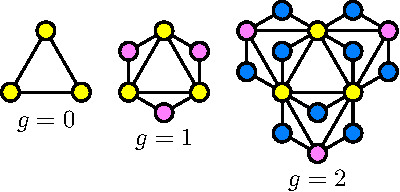
\includegraphics[width=0.75\linewidth]{Pseudofractal-eps-converted-to.pdf}
    \caption{ Illustration of the first several iterations of the pseudofractal scale-free web. }
    \label{psfw1}
\end{figure}
%%%%%%%%%%%%%%%%%%%%%%%%%%%%%%%%%%%%%%%%%%%%%%%%%%%%%%%%%%


The Koch network is also built in an iterative way~\cite{XiLiZh15}. Let \(\mathcal{M}_{g}\) (\(g \geq 0\)) denote the Koch network after \(g\) iterations. Initially (\(g=0\)), \(\mathcal{M}_{0}\) is a triangle with three
vertices and three edges. For \(g\geq 1\), \(\mathcal{M}_{g}\) is obtained from \(\mathcal{M}_{g-1}\) by
performing the following operations. For each of the three vertices in
every existing triangle in \(\mathcal{M}_{g-1}\), two new vertices are created, both of which and their
``mother'' vertices are connected to one another forming a new triangle. \figref{network} illustrates the growth process of the Koch network.  In network \(\mathcal{M}_{g}\), the number of vertices is \(2\times 4^{g}+1\), and the number of
edges is \(3\times 4^{g}\).  In~\cite{XiLiZh15}, the Kemeny constant \(K(\mathcal{M}_g)\) for \(\mathcal{M}_g\) was obtained to be
\begin{equation}\label{Kg02}
    K(\mathcal{M}_g)=(1+2g)\times 4^g+\frac{1}{3}\,. %\notag
\end{equation}

%%%%%%%%%%%%%%%%%%%%%%%%%%%%%%%%%%%%%%%%%%%%%%%%%%%%%%%%%
% Figure 2
%%%%%%%%%%%%%%%%%%%%%%%%%%%%%%%%%%%%%%%%%%%%%%%%%%%%%
\begin{figure}[!t]
    \centering
    % \includegraphics[width=0.85\linewidth,trim=0 0 0 0]{Koch.eps}
    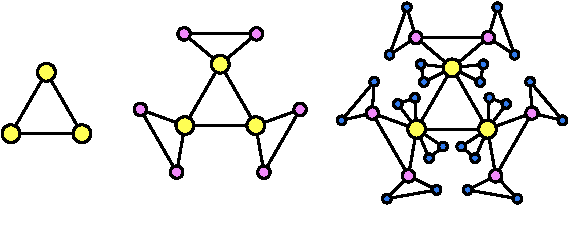
\includegraphics[width=0.85\linewidth]{Koch-eps-converted-to.pdf}
    \caption{Construction process for the Koch network.}
    \label{network}
\end{figure}
%%%%%%%%%%%%%%%%%%%%%%%%%%%%%%%%%%%%%%%%%%%%%%%%%%%%%

Let \(\mathcal{C}_{b,g}(b\ge3,g\ge0)\) represent the Cayley tree after
\(g\) iterations, which are constructed  as follows~\cite{CaCh97,ChCa99}. Initially \((g = 0)\), \(\mathcal{C}_{b,0}\) only contains a central vertex. To obtain \(\mathcal{C}_{b,1}\), we generate  \(b\) vertices and linked them to
the central one. For any \(g>1\), \(\mathcal{C}_{b,g}\) is obtained from \(\mathcal{C}_{b,g-1}\) by performing the following operation. For every periphery vertex of \(\mathcal{C}_{b,g-1}\), \(b-1\) vertices are created and connected to
the periphery vertex. \figref{Cayley} illustrates a special Cayley tree,
\(\mathcal{C}_{3,5}\). In the tree \(\mathcal{C}_{b,g}\), there are \((b(b-1)^g-2)/(b-2)\) vertices and \((b(b-1)^g-2)/(b-2)-1\) edges. In~\cite{JuWuZh13}, the authors  considered a particular Cayley tree \(\mathcal{C}_{3,g}\) corresponding to \(b=3\) and obtained an exact expression for its  Kemeny constant \(K(\mathcal{C}_{3,g})\):
\begin{equation}\label{Kg03}
    K(\mathcal{C}_{3,g})=\frac{3g\times 4^{g+1}-13\times 2^{2g+1} + 35\times 2^g - 9}{2(2^g-1)}.
\end{equation}

%%%%%%%%%%%%%%%%%%%%%%%%%%%%%%%%%%%%%%%%%%%%%%%%%%%%%%%%%
% Figure 3
%%%%%%%%%%%%%%%%%%%%%%%%%%%%%%%%%%%%%%%%%%%%%%%%%%%%%
\begin{figure}[!t]
    \centering
    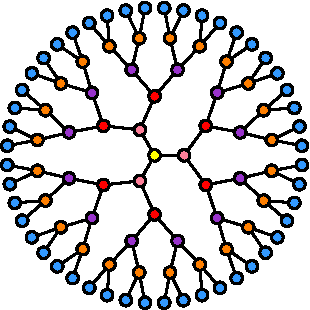
\includegraphics[width=0.6\linewidth,trim=0 0 0 0]{Cayley.pdf}
    %\includegraphics[width=0.5\textwidth]{Labelling.eps}
    \caption{The Cayley tree \(\mathcal{C}_{3,5}\).}
    \label{Cayley}
\end{figure}
%%%%%%%%%%%%%%%%%%%%%%%%%%%%%%%%%%%%%%%%%%%%%%%%%%%%%

\subsubsection{Extended Tower of Hanoi graphs}

As the name suggests, the extended Tower of Hanoi graph is constructed  based on the Tower of Hanoi graph.  Let \(\mathcal{H}_{g}\)  be the  Tower of Hanoi graph of generation \(g\)~\cite{HiKlMiPeSt13}. The vertex set of \(\mathcal{H}_{g}\) consists of all \(3\)-tuples of integers \(1,2,3\), i.e., \(V(\mathcal{H}_{g})=\{1,2,3\}^g\). All vertices in \(\mathcal{H}_{g}\) are labelled as \((x_1,x_2,\cdots,x_g)\), hereafter written in regular expression form \(x_1x_2\cdots x_g\), with \(x_i\in\{1,2,3\}\) for \(i=1,2,...,g\). Two vertices \(u=u_1u_2\cdots u_g\) and \(v=v_1v_2\cdots v_g\) in \(\mathcal{H}_{g}\) are directly connected by an edge if and only if there exists an \(h(1\le h\le g)\) such that
\begin{enumerate}
    \item \(u_t=v_t\) for \(1\le t\le h-1\);
    \item \(u_h\neq v_h\);
    \item \(u_t=v_h\) and \(v_t=u_h\) for \(h+1\le t\le g\).
\end{enumerate}

Figure~\ref{Sierpinski} illustrates the  Tower of Hanoi graph \(\mathcal{H}_{3}\) and its vertex labeling. In \(\mathcal{H}_{g}\), a vertex having label form \((ii\cdots i)(1\le i\le 3)\) is called an extreme vertex.

%%%%%%%%%%%%%%%%%%%%%%%%%%%%%%%%%%%%%%%%%%%%%%%%%%%%%%%%%
% Figure 4
%%%%%%%%%%%%%%%%%%%%%%%%%%%%%%%%%%%%%%%%%%%%%%%%%%%%%

\begin{figure}[!t]
    \centering
    \subfigure[\(\mathcal{H}_{3}\)]{
        \begin{minipage}[t]{0.5\linewidth}
            \centering
            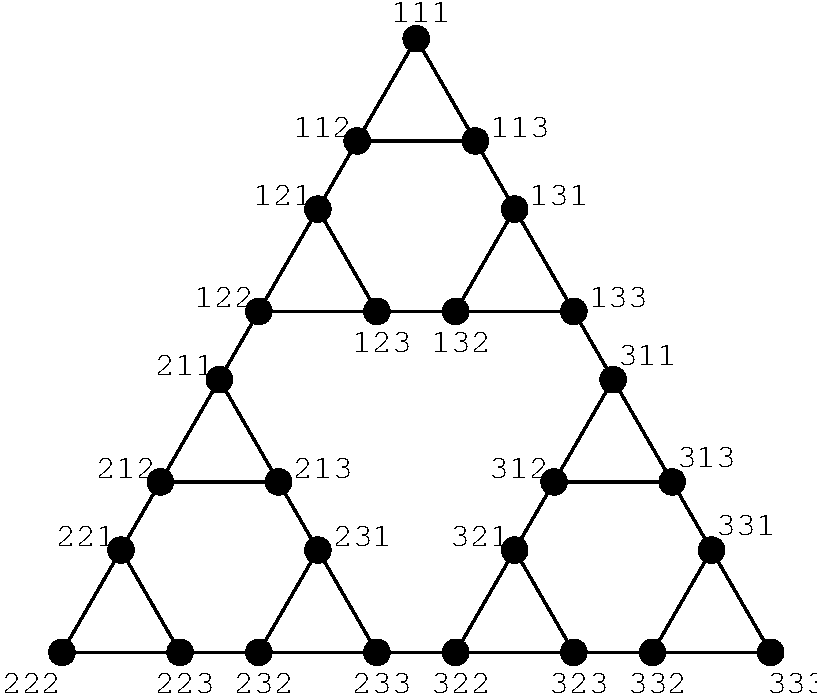
\includegraphics[width=0.95\linewidth,trim=0 0 0 0]{spsk.pdf}
            %\caption{The Sierpi\'nski graph \(\calS_{3,3}\) and its vertex labeling.}
            \label{Sierpinski}
        \end{minipage}%
    }%
    \subfigure[\(\overline{\mathcal{H}}_{3}\)]{
        \begin{minipage}[t]{0.5\linewidth}
            \centering
            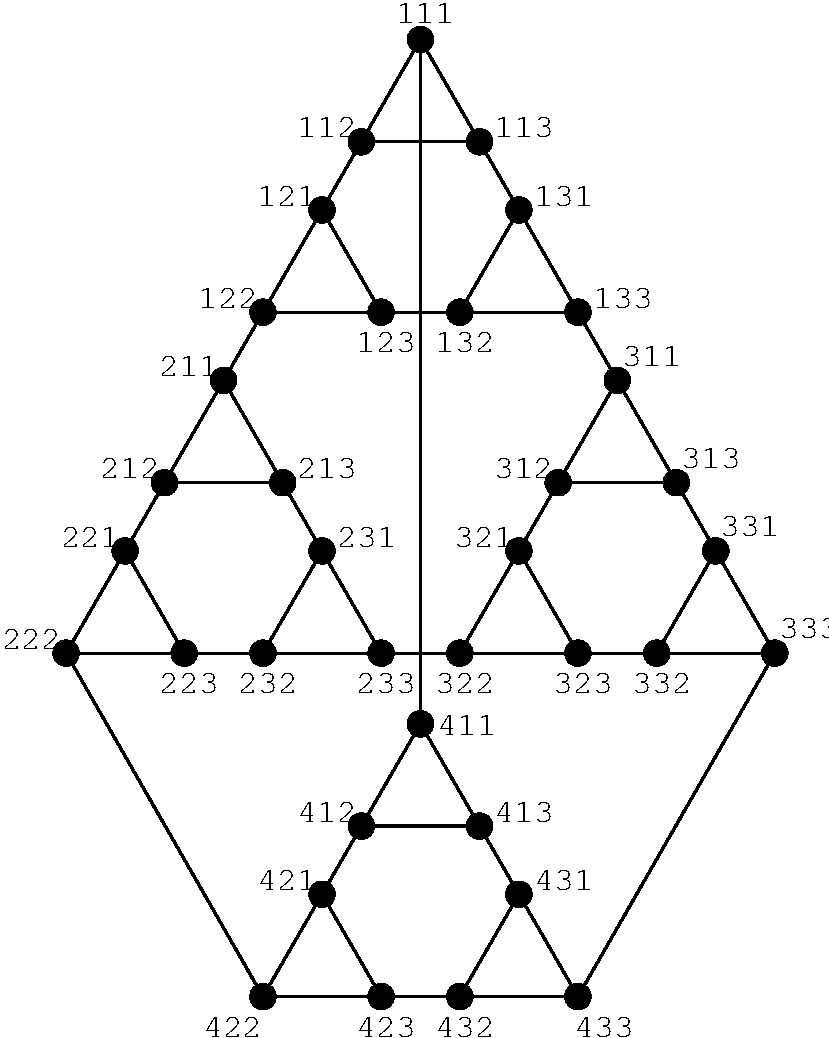
\includegraphics[width=0.95\linewidth,trim=0 0 0 0]{spsklk.pdf}
            %\caption{The extended Sierpi\'nski graph \(\calS^{++}_{3,3}\) and its vertex labeling.}
            \label{exSierpinski}
        \end{minipage}%
    }%
    \centering
    \caption{Illustrations of the Tower of Hanoi graph \(\mathcal{H}_{3}\) and its extension \(\overline{\mathcal{H}}_{3}\), as well as  their vertex labeling.}
\end{figure}
%%%%%%%%%%%%%%%%%%%%%%%%%%%%%%%%%%%%%%%%%%%%%%%%%%%%%

The extended  Tower of Hanoi graph denoted by \(\overline{\mathcal{H}}_{g}(g\ge 1)\)  proposed by Klava\u zar and Mohar~\cite{KlMo05}, is defined as follows. For \(g=1\), \(\overline{\mathcal{H}}_{1}\) is a triangle. For \(g\ge2\),  \(\overline{\mathcal{H}}_{g}\) was obtained from the disjoint union of \(4\) copies of \(\mathcal{H}_{g-1}\), where the extreme vertices in different  replicas of \(\mathcal{H}_{g-1}\) are connected as the 4-vertex complete graph. Figure~\ref{exSierpinski} shows the extended  Tower of Hanoi graph \(\overline{\mathcal{H}}_{3}\) and the its labeling. In graph \(\overline{\mathcal{H}}_{g}\), the number of nodes is \(4\cdot3^{g-1}\), and the number of edges is \(4\cdot3^g/2\). As shown in~\cite{QiZh18}, the Kemeny constant \(K(\overline{\mathcal{H}}_{g})\) for \(\overline{\mathcal{H}}_{g}\) is
\begin{align}
    K(\overline{\mathcal{H}}_{g}) = \frac{32\times5^g\times3^{g-1}-64\times3^{2g-2}-2\times3^g}{10(3^g+3^{g-1}-1)}.
    \label{Kg04}
\end{align}

We use our algorithm \(\text{Approx}\mathcal{HK}\) to compute the Kemeny constant on   pseudofractal scale-free web \(\mathcal{F}_{12}\),  Koch network \(\mathcal{M}_{10}\),   Cayley tree \(\mathcal{C}_{3,19}\), and   extended  Tower of Hanoi graph \(\overline{\mathcal{H}}_{13}\). The numerical results are reported in  Table~\ref{tab:Kemeny}, which shows that the approximation algorithm \(\text{Approx}\mathcal{HK}\) works effectively for the four  networks. This again demonstrates the advantage of our proposed algorithm for large networks.

\begin{table*}[htbp]
    %\tabcolsep=5pt
    \centering
    \normalsize
    %\fontsize{6.51}{8.0}\selectfont
    \begin{threeparttable}
        \caption{Exact Kemeny constant \(K\),   their approximation \(\tilde{K}\),  relative error \(\rho=\abs{K-\tilde{K}}/K\), and running time (seconds, \(s\)) for \(\tilde{K}\) on networks \(\mathcal{F}_{12}\) and \(\mathcal{M}_{10}\).  \(K\) is obtained via~\eqref{Kg01} and~\eqref{Kg02}, while \(\tilde{K}\) is obtained through algorithm \(\text{Approx}\mathcal{HK}\) with \(\epsilon=0.2\).}
        \label{tab:Kemeny}
        \begin{tabular}{ccccccc}
            \toprule
            Network                         & Vertices  & Edges     & \(K\)       & \(\tilde{K}\) & Error \(\rho\) & Time\cr
            \midrule
            \specialrule{0em}{3pt}{3pt}
            \(\mathcal{F}_{12}\)            & 797,163   & 1,594,323 & 1,321,776   & 1,322,243     & 0.00035        & 16.71\cr
            \specialrule{0em}{3pt}{3pt}
            \(\mathcal{M}_{10}\)            & 2,097,153 & 3,145,728 & 22,020,096  & 22,015,912    & 0.00004        & 45.70\cr
            \specialrule{0em}{3pt}{3pt}
            \(\mathcal{C}_{3,19}\)          & 1,572,862 & 1,572,861 & 52,953,206  & 52,564,893    & 0.00733        & 31.48\cr
            \specialrule{0em}{3pt}{3pt}
            \(\overline{\mathcal{H}}_{13}\) & 2,125,764 & 3,188,646 & 975,712,653 & 970,030,470   & 0.00582        & 1028\cr
            \specialrule{0em}{3pt}{3pt}
            \bottomrule
        \end{tabular}
    \end{threeparttable}
\end{table*}

\subsection{Results for \textsc{ExactAGCM} and \textsc{ApproxAGCM}}

We first compare the performance of \textsc{ExactAGCM} and \textsc{ApproxAGCM} with the optimum solution on four toy networks~\cite{Ku13}: \(\mathit{Zebra}\) with 23 vertices, \(\mathit{Zachary\ karate\ club}\) with 34 vertices, \(\mathit{Contiguous\ USA}\) with 49 vertices and \(\mathit{Les\ Miserables}\) with 77 vertices.

To find the set of \(k\) elements with the lowest AGC value for each network \(\gr=(V,E)\), the optimum solution iterates through all the \(k\)-element subsets of \(V\), where \(k\) ranges from \(1\) to \(5\).
We then compare the smallest AGC value with the solution provided by \textsc{ExactAGCM} and \textsc{ApproxAGCM}, whose results are shown in \figref{pic:compare-effect-optimum}.
During the execution of \textsc{ApproxAGCM}, we set the error parameter \(\epsilon\) to \(0.2\).
The results in \figref{pic:compare-effect-optimum} demonstrate that the solutions provided by our algorithms are almost identical to each other, and both are very close to the optimum solution.
This indicates that our proposed algorithms have a much better approximation ratio than the theoretical guarantees.

\begin{figure}[!t]
    \centering
    \begin{tikzpicture}[scale=\scaleoptimum,baseline]
        \begin{axis}[
                xlabel=\Large{\(k\)},
                ylabel=\Large{\(H(S)\)},
                legend style={font=\Large},
                legend entries={ApproxAGCM,ExactAGCM,OptimumAGCM},
            ]
            \addplot+[
                mark=pentagon*,
                mark size = 3pt
            ] table {compare_effects/optimum/Zebra/Approx.dat};
            \addplot table {compare_effects/optimum/Zebra/Exact.dat};
            \addplot table {compare_effects/optimum/Zebra/Optimum.dat};
            \node [font=\huge] at (3.5,10) {(a)};
        \end{axis}
    \end{tikzpicture}
    \begin{tikzpicture}[scale=\scaleoptimum,baseline]
        \begin{axis}[
                xlabel=\Large{\(k\)},
                ylabel=\Large{\(H(S)\)},
                legend style={font=\Large},
                legend entries={ApproxAGCM,ExactAGCM,OptimumAGCM},
            ]
            \addplot+[
                mark=pentagon*,
                mark size = 3pt
            ] table {compare_effects/optimum/Zachary karate club/Approx.dat};
            \addplot table {compare_effects/optimum/Zachary karate club/Exact.dat};
            \addplot table {compare_effects/optimum/Zachary karate club/Optimum.dat};
            \node [font=\huge] at (3.5,7) {(b)};
        \end{axis}
    \end{tikzpicture}

    \begin{tikzpicture}[scale=\scaleoptimum,baseline]
        \begin{axis}[
                xlabel=\Large{\(k\)},
                ylabel=\Large{\(H(S)\)},
                legend style={font=\Large},
                legend entries={ApproxAGCM,ExactAGCM,OptimumAGCM},
            ]
            \addplot+[
                mark=pentagon*,
                mark size = 3pt
            ] table {compare_effects/optimum/Contiguous USA/Approx.dat};
            \addplot table {compare_effects/optimum/Contiguous USA/Exact.dat};
            \addplot table {compare_effects/optimum/Contiguous USA/Optimum.dat};
            \node [font=\huge] at (3.5,25) {(c)};
        \end{axis}
    \end{tikzpicture}
    \begin{tikzpicture}[scale=\scaleoptimum,baseline]
        \begin{axis}[
                xlabel=\Large{\(k\)},
                ylabel=\Large{\(H(S)\)},
                legend style={font=\Large},
                legend entries={ApproxAGCM,ExactAGCM,OptimumAGCM},
            ]
            \addplot+[
                mark=pentagon*,
                mark size = 3pt
            ] table {compare_effects/optimum/Les Miserables/Approx.dat};
            \addplot table {compare_effects/optimum/Les Miserables/Exact.dat};
            \addplot table {compare_effects/optimum/Les Miserables/Optimum.dat};
            \node [font=\huge] at (3.5,9) {(d)};
        \end{axis}
    \end{tikzpicture}
    \caption{AGC \(\manc{S}\) of vertex group \(S\) computed by three different algorithms(\textsc{ExactAGCM},\textsc{ApproxAGCM} and \textsc{OptimumAGCM}) on four networks: Zebra (a), Zachary karate club (b), Contiguous USA (c) and Les Miserables (d).\label{pic:compare-effect-optimum}}
\end{figure}

We then compare the performance of \textsc{ExactAGCM} and \textsc{ApproxAGCM} with three other algorithms: \textsc{Top-Absorb}, \textsc{Top-Degree}, and \textsc{Top-PageRank}.
\textsc{Top-Absorb} simply selects \(k\) absorbing vertices with the lowest absorbing random-walk centrality, while \textsc{Top-Degree} and \textsc{Top-PageRank} select the vertices with the largest degrees and PageRank values, respectively.
We execute these four algorithms on eight medium-sized networks, and the results are shown in \figref{pic:compare-effect1} and \figref{pic:compare-effect2}.
As displayed in \figref{pic:compare-effect1} and \figref{pic:compare-effect2}, both of our algorithms produce similar approximate solutions in larger networks, which outperform the solutions of other algorithms.

\begin{figure}[!t]
    \centering
    \begin{tikzpicture}[scale=\scaleexact,baseline]
        \begin{semilogyaxis}[
                xlabel=\Large{\(k\)},
                ylabel=\Large{\(H(S)\)},
                minor x tick num=1,
                minor y tick num=4,
                legend style={
                        font=\footnotesize,
                        legend columns=2,
                    },
                legend entries={ApproxAGCM,ExactAGCM,Top-Absorb,Top-Degree,Top-PageRank},
                ymax=800,
            ]
            \addplot+[
                mark=pentagon*,
                mark size = 3pt
            ] table {compare_effects/exact/CA-GrQc/Approx.dat};
            \addplot table {compare_effects/exact/CA-GrQc/Exact.dat};
            \addplot table {compare_effects/exact/CA-GrQc/Top-Absorb.dat};
            \addplot table {compare_effects/exact/CA-GrQc/Top-Degree.dat};
            \addplot table {compare_effects/exact/CA-GrQc/Top-PageRank.dat};
            \node [font=\huge] at (10,30) {(a)};
        \end{semilogyaxis}
    \end{tikzpicture}
    \begin{tikzpicture}[scale=\scaleexact,baseline]
        \begin{semilogyaxis}[
                xlabel=\Large{\(k\)},
                ylabel=\Large{\(H(S)\)},
                minor x tick num=1,
                minor y tick num=4,
                legend style={
                        font=\footnotesize,
                        legend columns=2,
                    },
                legend entries={ApproxAGCM,ExactAGCM,Top-Absorb,Top-Degree,Top-PageRank},
                ymax=4500,
            ]
            \addplot+[
                mark=pentagon*,
                mark size = 3pt
            ] table {compare_effects/exact/ego-Facebook/Approx.dat};
            \addplot table {compare_effects/exact/ego-Facebook/Exact.dat};
            \addplot table {compare_effects/exact/ego-Facebook/Top-Absorb.dat};
            \addplot table {compare_effects/exact/ego-Facebook/Top-Degree.dat};
            \addplot table {compare_effects/exact/ego-Facebook/Top-PageRank.dat};
            \node [font=\huge] at (10,20) {(b)};
        \end{semilogyaxis}
    \end{tikzpicture}

    \begin{tikzpicture}[scale=\scaleexact,baseline]
        \begin{semilogyaxis}[
                xlabel=\Large{\(k\)},
                ylabel=\Large{\(H(S)\)},
                ytick distance=10^1,
                minor x tick num=1,
                minor y tick num=4,
                legend style={
                        font=\footnotesize,
                        legend columns=2,
                    },
                legend entries={ApproxAGCM,ExactAGCM,Top-Absorb,Top-Degree,Top-PageRank},
                ymax=1600,
            ]
            \addplot+[
                mark=pentagon*,
                mark size = 3pt
            ] table {compare_effects/exact/Euroroads/Approx.dat};
            \addplot table {compare_effects/exact/Euroroads/Exact.dat};
            \addplot table {compare_effects/exact/Euroroads/Top-Absorb.dat};
            \addplot table {compare_effects/exact/Euroroads/Top-Degree.dat};
            \addplot table {compare_effects/exact/Euroroads/Top-PageRank.dat};
            \node [font=\huge] at (10,25) {(c)};
        \end{semilogyaxis}
    \end{tikzpicture}
    \begin{tikzpicture}[scale=\scaleexact,baseline]
        \begin{semilogyaxis}[
                xlabel=\Large{\(k\)},
                ylabel=\Large{\(H(S)\)},
                minor x tick num=1,
                minor y tick num=4,
                legend style={
                        font=\footnotesize,
                        legend columns=2,
                    },
                legend entries={ApproxAGCM,ExactAGCM,Top-Absorb,Top-Degree,Top-PageRank},
                ymax=12000,
            ]
            \addplot+[
                mark=pentagon*,
                mark size = 3pt
            ] table {compare_effects/exact/US power grid/Approx.dat};
            \addplot table {compare_effects/exact/US power grid/Exact.dat};
            \addplot table {compare_effects/exact/US power grid/Top-Absorb.dat};
            \addplot table {compare_effects/exact/US power grid/Top-Degree.dat};
            \addplot table {compare_effects/exact/US power grid/Top-PageRank.dat};
            \node [font=\huge] at (10,90) {(d)};
        \end{semilogyaxis}
    \end{tikzpicture}
    \caption{AGC \(\manc{S}\) of vertex group \(S\) computed by four different algorithms(\textsc{ExactAGCM},\textsc{ApproxAGCM},\textsc{Top-Absorb} and \textsc{Top-Degree}) on four networks: CA-GrQc (a), ego-Facebook (b), Euroroads (c) and US power grid (d).\label{pic:compare-effect1}}
\end{figure}

\begin{figure}[!t]
    \centering
    \begin{tikzpicture}[scale=\scaleexact,baseline]
        \begin{semilogyaxis}[
                xlabel=\Large{\(k\)},
                ylabel=\Large{\(H(S)\)},
                minor x tick num=1,
                minor y tick num=4,
                legend style={
                        font=\footnotesize,
                        legend columns=2,
                    },
                legend entries={ApproxAGCM,ExactAGCM,Top-Absorb,Top-Degree,Top-PageRank},
                % ymax=800,
            ]
            \addplot+[
                mark=pentagon*,
                mark size = 3pt
            ] table {compare_effects/exact/Hamsterster friends/Approx.dat};
            \addplot table {compare_effects/exact/Hamsterster friends/Exact.dat};
            \addplot table {compare_effects/exact/Hamsterster friends/Top-Absorb.dat};
            \addplot table {compare_effects/exact/Hamsterster friends/Top-Degree.dat};
            \addplot table {compare_effects/exact/Hamsterster friends/Top-PageRank.dat};
            \node [font=\huge] at (15,7) {(a)};
        \end{semilogyaxis}
    \end{tikzpicture}
    \begin{tikzpicture}[scale=\scaleexact,baseline]
        \begin{semilogyaxis}[
                xlabel=\Large{\(k\)},
                ylabel=\Large{\(H(S)\)},
                minor x tick num=1,
                minor y tick num=4,
                legend style={
                        font=\footnotesize,
                        legend columns=2,
                    },
                legend entries={ApproxAGCM,ExactAGCM,Top-Absorb,Top-Degree,Top-PageRank},
                % ymax=4500,
            ]
            \addplot+[
                mark=pentagon*,
                mark size = 3pt
            ] table {compare_effects/exact/Hamsterster full/Approx.dat};
            \addplot table {compare_effects/exact/Hamsterster full/Exact.dat};
            \addplot table {compare_effects/exact/Hamsterster full/Top-Absorb.dat};
            \addplot table {compare_effects/exact/Hamsterster full/Top-Degree.dat};
            \addplot table {compare_effects/exact/Hamsterster full/Top-PageRank.dat};
            \node [font=\huge] at (15,10) {(b)};
        \end{semilogyaxis}
    \end{tikzpicture}

    \begin{tikzpicture}[scale=\scaleexact,baseline]
        \begin{semilogyaxis}[
                xlabel=\Large{\(k\)},
                ylabel=\Large{\(H(S)\)},
                ytick distance=10^1,
                minor x tick num=1,
                minor y tick num=4,
                legend style={
                        font=\footnotesize,
                        legend columns=2,
                    },
                legend entries={ApproxAGCM,ExactAGCM,Top-Absorb,Top-Degree,Top-PageRank},
                % ymax=1600,
            ]
            \addplot+[
                mark=pentagon*,
                mark size = 3pt
            ] table {compare_effects/exact/Reactome/Approx.dat};
            \addplot table {compare_effects/exact/Reactome/Exact.dat};
            \addplot table {compare_effects/exact/Reactome/Top-Absorb.dat};
            \addplot table {compare_effects/exact/Reactome/Top-Degree.dat};
            \addplot table {compare_effects/exact/Reactome/Top-PageRank.dat};
            \node [font=\huge] at (15,25) {(c)};
        \end{semilogyaxis}
    \end{tikzpicture}
    \begin{tikzpicture}[scale=\scaleexact,baseline]
        \begin{semilogyaxis}[
                xlabel=\Large{\(k\)},
                ylabel=\Large{\(H(S)\)},
                minor x tick num=1,
                minor y tick num=4,
                legend style={
                        font=\footnotesize,
                        legend columns=2,
                    },
                legend entries={ApproxAGCM,ExactAGCM,Top-Absorb,Top-Degree,Top-PageRank},
                % ymax=12000,
            ]
            \addplot+[
                mark=pentagon*,
                mark size = 3pt
            ] table {compare_effects/exact/Route views/Approx.dat};
            \addplot table {compare_effects/exact/Route views/Exact.dat};
            \addplot table {compare_effects/exact/Route views/Top-Absorb.dat};
            \addplot table {compare_effects/exact/Route views/Top-Degree.dat};
            \addplot table {compare_effects/exact/Route views/Top-PageRank.dat};
            \node [font=\huge] at (15,4) {(d)};
        \end{semilogyaxis}
    \end{tikzpicture}
    \caption{AGC \(\manc{S}\) of vertex group \(S\) computed by four different algorithms(\textsc{ExactAGCM},\textsc{ApproxAGCM},\textsc{Top-Absorb} and \textsc{Top-Degree}) on four networks: Hamster friends (a), Hamster full (b), Reactome (c) and Route views (d).\label{pic:compare-effect2}}
\end{figure}

Finally, we demonstrate that the \textsc{ApproxAGCM} algorithm is significantly more efficient than the \textsc{ExactAGCM} algorithm, particularly when applied to large networks.
We test both algorithms on a wider range of real networks.
For each network, we use \textsc{ExactAGCM} and \textsc{ApproxAGCM} separately to solve the AGC minimization problem, with \(k=10\) and \(\epsilon=0.2\).
The running times of both algorithms are shown in \tabref{tab:running-time}.

From \tabref{tab:running-time}, we can observe that the running time of \textsc{ApproxAGCM} is proportional to the number of edges in the network, leading to an increase in the speedup ratio of \textsc{ApproxAGCM} as the network size grows.
Furthermore, \tabref{tab:running-time} indicates that when processing networks marked with \(\ast\),
\textsc{ApproxAGCM} remains usable while \textsc{ExactAGCM} fails due to its high time complexity.
This result demonstrates the scalability of \text{ApproxAGCM} when applied to large networks.

\begin{table}[htbp]
    \tabcolsep=8pt
    \centering
    \fontsize{8.0}{8.8}\selectfont
    \begin{threeparttable}
        \caption{The running time (seconds, \(s\)) of \textsc{ExactAGCM} and \textsc{ApproxAGCM} (denoted as \textsc{Exact} and \textsc{Approx} in the table to save space) with various \(\epsilon\) on several realistic networks}
        \label{tab:running-time}
        \begin{tabularx}{8.25cm}{c p{1cm} p{0.5cm} p{0.5cm} p{0.5cm}}
            \toprule[1pt]
            \multirow{2}{*}{Network}        &
            \multirow{2}{*}{\textsc{Exact}} &
            \multicolumn{3}{c}{\textsc{Approx} for various \(\epsilon\)}\cr
            \cmidrule{3-5}
                                            & (\(s\)) & \(0.3\) & \(0.25\) & \(0.2\)\cr
            \midrule
            Jazz musicians                  & 0.214   & 0.157   & 0.178    & 0.194\cr
            Euroroads                       & 0.498   & 0.239   & 0.277    & 0.281\cr
            Hamster friends                 & 1.183   & 0.348   & 0.450    & 0.629\cr
            Hamster full                    & 1.267   & 0.402   & 0.525    & 1.049\cr
            Facebook (NIPS)                 & 10.20   & 1.956   & 2.919    & 4.349\cr
            CA-GrQc                         & 10.74   & 0.686   & 0.896    & 0.968\cr
            US power grid                   & 17.62   & 0.500   & 0.634    & 0.977\cr
            Reactome                        & 30.13   & 3.593   & 4.680    & 7.329\cr
            Route views                     & 37.55   & 0.582   & 0.704    & 1.024\cr
            CA-HepTh                        & 85.83   & 1.108   & 1.602    & 2.476\cr
            Sister cities                   & 143.3   & 3.246   & 3.974    & 7.013\cr
            Pretty Good Privacy             & 157.7   & 3.844   & 5.170    & 7.657\cr
            CA-HepPh                        & 180.8   & 6.601   & 9.775    & 15.74\cr
            Astro-ph                        & 715.8   & 13.51   & 18.26    & 31.31\cr
            CAIDA                           & 2272    & 6.355   & 7.838    & 11.28\cr
            Brightkite*                     & --      & 23.31   & 32.68    & 54.21\cr
            Livemocha*                      & --      & 177.0   & 250.6    & 392.1\cr
            WordNet*                        & --      & 83.89   & 124.5    & 221.4\cr
            Gowalla*                        & --      & 129.1   & 195.7    & 342.8\cr
            com-DBLP*                       & --      & 232.7   & 399.1    & 756.8\cr
            Amazon*                         & --      & 349.5   & 652.3    & 1082\cr
            roadNet-PA*                     & --      & 2215    & 3349     & 5714\cr
            YouTube*                        & --      & 1482    & 2197     & 3661\cr
            roadNet-TX*                     & --      & 3135    & 4464     & 9338\cr
            roadNet-CA*                     & --      & 5445    & 8214     & 14458\cr
            \bottomrule
        \end{tabularx}
    \end{threeparttable}
\end{table}

\section{Conclusions}

The hitting time of random walks arises in many practical scenarios.
However, exactly computing the hitting time is prohibitively expensive, making it difficult to solve corresponding optimization problems.
In this paper, we studied absorbing random-walk centrality and Kemeny constant of a graph, both of which are actually weighted average of hitting times and have found wide applications.
We established a link between the two quantities and reformulated them in terms of quadratic forms of the pseudoinverse of graph Laplacian.
Subsequently, we extended the notion of mean hitting time to multiple vertices, proposing Absorbing Group Centrality (AGC) and its minimization problem.
We demonstrated the monotonicity and supermodularity of this newly proposed centrality, expressing it in terms of the inverse of a SDDM matrix.
Moreover, we provided a randomized approximation algorithm with probabilistic guarantee, which computes the walk centrality for all vertices and Kemeny constant in nearly linear time with respect to the number of edges.
Based on this algorithm, we provided another nearly linear greedy approximate algorithm to solve the minimization problem of AGC, which is proved to be NP-hard.
Finally, we conducted extensive experiments on various real-world and model networks, which show that the proposed algorithms are both efficient and accurate, especially for large-scale networks.

\bibliographystyle{IEEEtran}
\balance
\bibliography{refs}

\begin{IEEEbiography}[\biophoto{xhs.jpg}]{Haisong Xia}
    received the B.S. degree in computer science from Fudan University, Shanghai, China, in 2022. He is currently pursuing the master's degree in the School of Computer Science at Fudan University.
    His current research interests include network science, spectral graph theory and social network analysis.
\end{IEEEbiography}

\begin{IEEEbiography}{Wanyue Xu}
    (Student Member, IEEE) received the B.Eng. degree in computer science and technology from Shangdong University, Weihai, China, in 2019. She is currently pursuing the master's degree with the School of Computer Science, Fudan University, Shanghai, China.
    Her research interests include network science, graph data mining, social network analysis, and random walks.
\end{IEEEbiography}

\begin{IEEEbiography}{Zuobai Zhang}
    received the B.S. degree  in computer science from Fudan University, Shanghai, China, in 2021. 	He is currently pursuing the Ph.D. degree at Mila - Qu\'{e}bec AI Institute, Canada. His research interests include graph algorithms, graph representation learning, and drug discovery.
\end{IEEEbiography}

\begin{IEEEbiography}{Zhuoqing Song}
    received the B.S. degree in mathematics and applied mathematics in 2019 from Fudan University, Shanghai, China, where he is currently working toward the Ph.D. degree in applied mathematics. His research interests include decentralized optimization, graph algorithms, and machine learning.
\end{IEEEbiography}

\begin{IEEEbiography}[\biophoto{zzz.jpg}]{Zhongzhi Zhang}
    (Member, IEEE) received the B.Sc. degree in applied mathematics from Anhui University, Hefei, China, in 1997 and the Ph.D. degree in management science and engineering from Dalian University of Technology, Dalian, China, in 2006. \\
    From 2006 to 2008, he was a Post-Doctoral Research Fellow with Fudan University, Shanghai, China, where he is currently a Full Professor with the School of Computer Science. He has published over 150 papers in international journals or conferences. He has over 3300 ISI Web of Science citations with an H-index of 33 according to the Clarivate. He was selected as one of the most cited Chinese researchers
    (Elsevier) in 2019 and 2020. His current research interests include network science, graph data mining, social network analysis, spectral graph theory, and random walks. \\
    Dr. Zhang was a recipient of the Excellent Doctoral Dissertation Award of Liaoning Province, China, in 2007, the Excellent Post-Doctor Award of Fudan University in 2008, the Shanghai Natural Science Award (third class) in 2013, and the Wilkes Award for the best paper published in The Computer Journal in 2019. He is a member of the IEEE.
\end{IEEEbiography}

\end{document}
